\chapter{Syntactic sugar, and computing every
function}\label{finiteuniversalchap}

\begin{objectives} \label[objectives]{Get-comfortable-with-synt}

\begin{itemize}
\tightlist
\item
  Get comfortable with syntactic sugar or automatic translation of
  higher level logic to low level gates.\\
\item
  Learn proof of major result: every finite function can be computed by
  a Boolean circuit.\\
\item
  Start thinking \emph{quantitatively} about number of lines required
  for computation.
\end{itemize}

\end{objectives}

\begin{quote}
\emph{``{[}In 1951{]} I had a running compiler and nobody would touch it
because, they carefully told me, computers could only do arithmetic;
they could not do programs.''}, Grace Murray Hopper, 1986.
\end{quote}

\begin{quote}
\emph{``Syntactic sugar causes cancer of the semicolon.''}, Alan Perlis,
1982.
\end{quote}

The computational models we considered thus far are as ``bare bones'' as
they come. For example, our NAND-CIRC ``programming language'' has only
the single operation \texttt{foo = NAND(bar,blah)}. In this chapter we
will see that these simple models are actually \emph{equivalent} to more
sophisticated ones. The key observation is that we can implement more
complex features using our basic building blocks, and then use these new
features themselves as building blocks for even more sophisticated
features. This is known as ``syntactic sugar'' in the field of
programming language design since we are not modifying the underlying
programming model itself, but rather we merely implement new features by
syntactically transforming a program that uses such features into one
that doesn't.

This chapter provides a ``toolkit'' that can be used to show that many
functions can be computed by NAND-CIRC programs, and hence also by
Boolean circuits. We will also use this toolkit to prove a fundamental
theorem: \emph{every} finite function
\(f:\{0,1\}^n \rightarrow \{0,1\}^m\) can be computed by a Boolean
circuit, see \cref{circuit-univ-thm} below. While the syntactic sugar
toolkit is important in its own right, \cref{circuit-univ-thm} can also
be proven directly without using this toolkit. We present this
alternative proof in \cref{seccomputalternative}. See
\cref{computefuncoverviewfig} for an outline of the results of this
chapter.


\begin{figure}
\centering
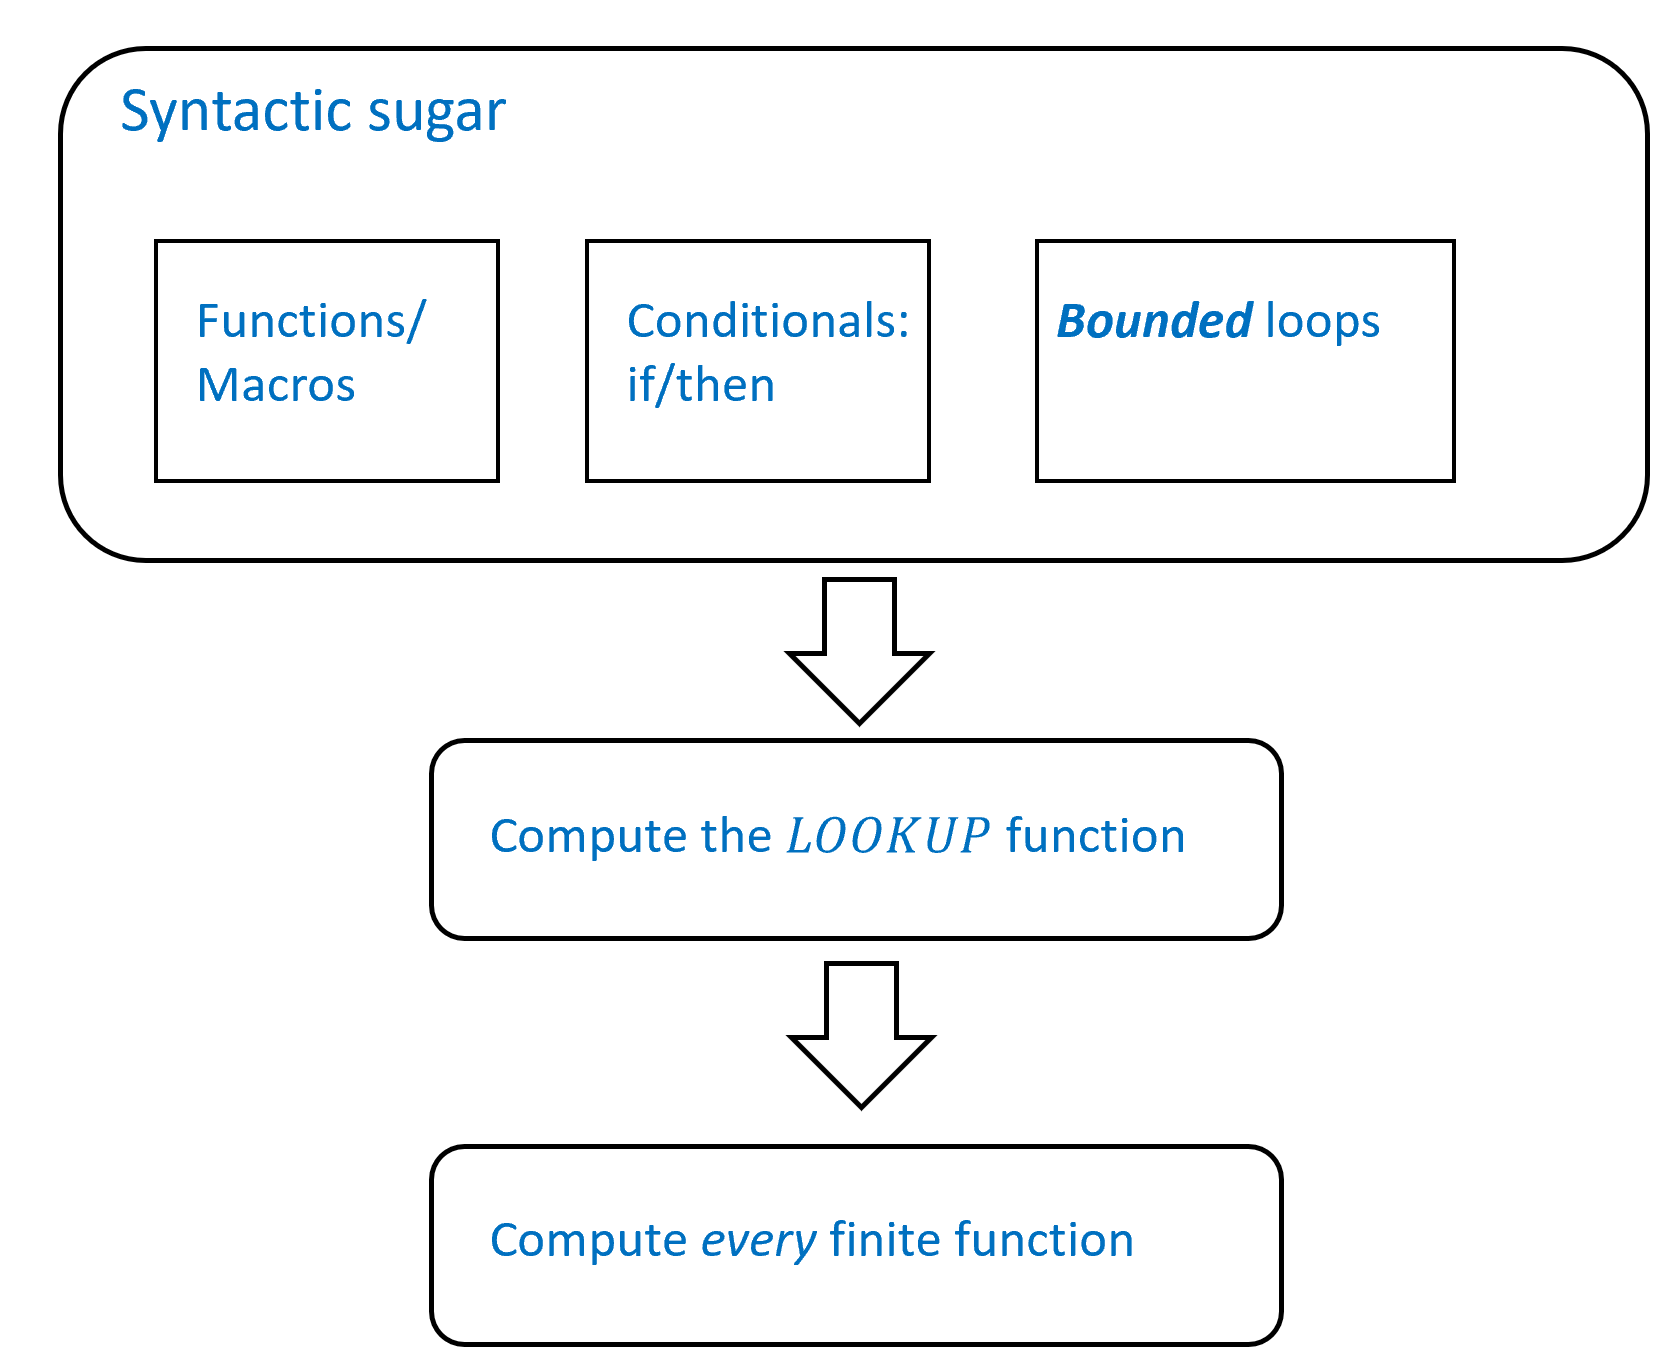
\includegraphics[width=\textwidth, height=0.25\paperheight, keepaspectratio]{../figure/compute_every_function_overview.png}
\caption{An outline of the results of this chapter. In
\cref{secsyntacticsugar} we give a toolkit of ``syntactic sugar''
transformations showing how to implement features such as
programmer-defined functions and conditional statements in NAND-CIRC. We
use these tools in \cref{seclookupfunc} to give a NAND-CIRC program (or
alternatively a Boolean circuit) to compute the
\(\ensuremath{\mathit{LOOKUP}}\) function. We then build on this result
to show in \cref{seccomputeallfunctions} that NAND-CIRC programs (or
equivalently, Boolean circuits) can compute \emph{every} finite
function. An alternative direct proof of the same result is given in
\cref{seccomputalternative}.}
\label{computefuncoverviewfig}
\end{figure}

\section{Some examples of syntactic sugar}\label{secsyntacticsugar}

We now present some examples of ``syntactic sugar'' transformations that
we can use in constructing straightline programs or circuits. We focus
on the \emph{straight-line programming language} view of our
computational models, and specifically (for the sake of concreteness) on
the NAND-CIRC programming language. This is convenient because many of
the syntactic sugar transformations we present are easiest to think
about in terms of applying ``search and replace'' operations to the
source code of a program. However, by \cref{equivalencemodelsthm}, all
of our results hold equally well for circuits, whether ones using NAND
gates or Boolean circuits that use the AND, OR, and NOT operations.
Enumerating the examples of such syntactic sugar transformations can be
a little tedious, but we do it for two reasons:

\begin{enumerate}
\def\labelenumi{\arabic{enumi}.}
\item
  To convince you that despite their seeming simplicity and limitations,
  simple models such as Boolean circuits or the NAND-CIRC programming
  language are actually quite powerful.
\item
  So you can realize how lucky you are to be taking a theory of
  computation course and not a compilers course\ldots{} \texttt{:)}
\end{enumerate}

\subsection{User-defined procedures}\label{User-defined-procedures}

One staple of almost any programming language is the ability to define
and then execute \emph{procedures} or \emph{subroutines}. (These are
often known as \emph{functions} in some programming languages, but we
prefer the name \emph{procedures} to avoid confusion with the function
that a program computes.) The NAND-CIRC programming language does not
have this mechanism built in. However, we can achieve the same effect
using the time honored technique of ``copy and paste''. Specifically, we
can replace code which defines a procedure such as

\begin{code}
def Proc(a,b):
    proc_code
    return c
some_code
f = Proc(d,e)
some_more_code
\end{code}

with the following code where we ``paste'' the code of \texttt{Proc}

\begin{code}
some_code
proc_code'
some_more_code
\end{code}

and where \texttt{proc\_code'} is obtained by replacing all occurrences
of \texttt{a} with \texttt{d}, \texttt{b} with \texttt{e}, and
\texttt{c} with \texttt{f}. When doing that we will need to ensure that
all other variables appearing in \texttt{proc\_code'} don't interfere
with other variables. We can always do so by renaming variables to new
names that were not used before. The above reasoning leads to the proof
of the following theorem:

\hypertarget{functionsynsugarthm}{}
\begin{theorem}[Procedure definition synctatic sugar] \label[theorem]{functionsynsugarthm}

Let NAND-CIRC-PROC be the programming language NAND-CIRC augmented with
the syntax above for defining procedures. Then for every NAND-CIRC-PROC
program \(P\), there exists a standard (i.e., ``sugar free'') NAND-CIRC
program \(P'\) that computes the same function as \(P\).

\end{theorem}

\hypertarget{norecursion}{}
\begin{remark}[No recursive procedure] \label[remark]{norecursion}

NAND-CIRC-PROC only allows \emph{non recursive} procedures. In
particular, the code of a procedure \texttt{Proc} cannot call
\texttt{Proc} but only use procedures that were defined before it.
Without this restriction, the above ``search and replace'' procedure
might never terminate and \cref{functionsynsugarthm} would not be true.

\end{remark}

\cref{functionsynsugarthm} can be proven using the transformation above,
but since the formal proof is somewhat long and tedious, we omit it
here.

\hypertarget{majcircnand}{}
\begin{example}[Computing Majority from NAND using syntactic sugar] \label[example]{majcircnand}

Procedures allow us to express NAND-CIRC programs much more cleanly and
succinctly. For example, because we can compute AND, OR, and NOT using
NANDs, we can compute the \emph{Majority} function as follows:

\begin{code}
def NOT(a):
    return NAND(a,a)
def AND(a,b):
    temp = NAND(a,b)
    return NOT(temp)
def OR(a,b):
    temp1 = NOT(a)
    temp2 = NOT(b)
    return NAND(temp1,temp2)

def MAJ(a,b,c):
    and1 = AND(a,b)
    and2 = AND(a,c)
    and3 = AND(b,c)
    or1 = OR(and1,and2)
    return OR(or1,and3)

print(MAJ(0,1,1))
# 1
\end{code}

\cref{progcircmajfig} presents the ``sugar free'' NAND-CIRC program (and
the corresponding circuit) that is obtained by ``expanding out'' this
program, replacing the calls to procedures with their definitions.

\end{example}

\hypertarget{synsugar}{}
\begin{bigidea} \label[bigidea]{synsugar}

Once we show that a computational model \(X\) is equivalent to a model
that has feature \(Y\), we can assume we have \(Y\) when showing that a
function \(f\) is computable by \(X\).

\end{bigidea}


\begin{figure}
\centering
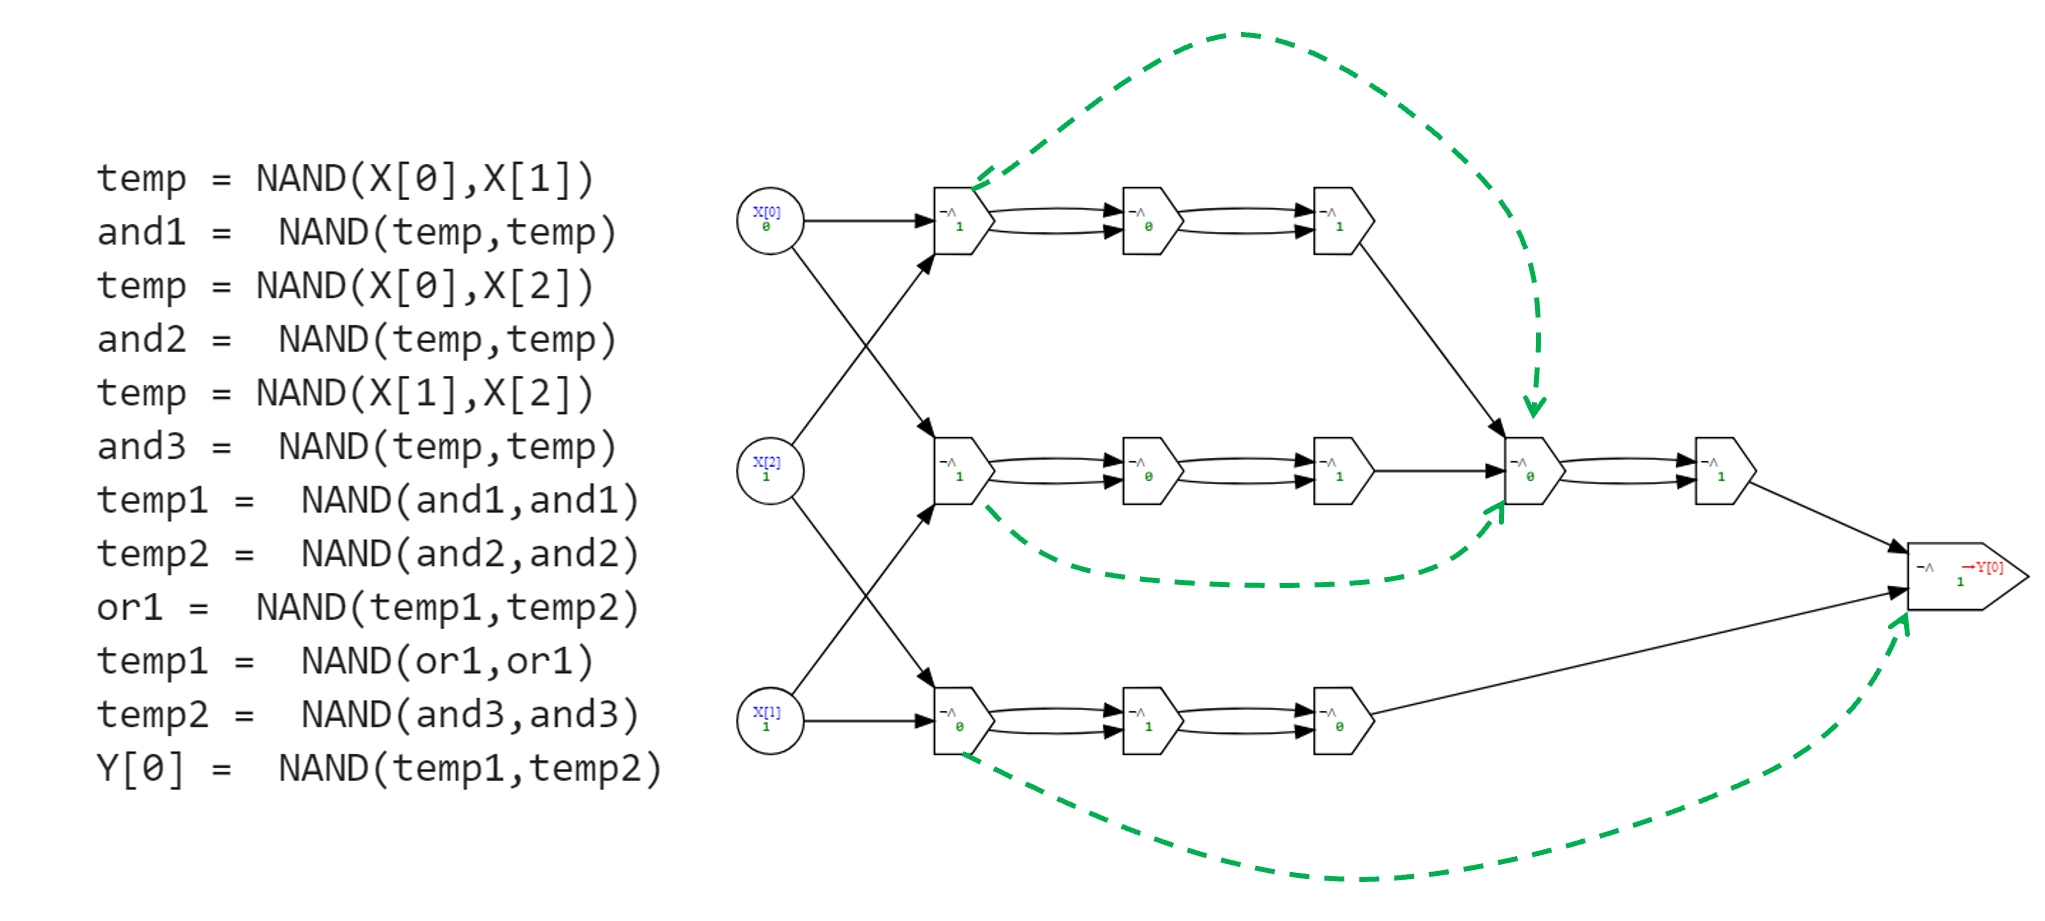
\includegraphics[width=\textwidth, height=0.25\paperheight, keepaspectratio]{../figure/progcircmaj.png}
\caption{A standard (i.e., ``sugar free'') NAND-CIRC program that is
obtained by expanding out the procedure definitions in the program for
Majority of \cref{majcircnand}. The corresponding circuit is on the
right. Note that this is not the most efficient NAND circuit/program for
majority: we can save on some gates by ``short cutting'' steps where a
gate \(u\) computes \(\ensuremath{\mathit{NAND}}(v,v)\) and then a gate
\(w\) computes \(\ensuremath{\mathit{NAND}}(u,u)\) (as indicated by the
dashed green arrows in the above figure).}
\label{progcircmajfig}
\end{figure}

\hypertarget{countinglines}{}
\begin{remark}[Counting lines] \label[remark]{countinglines}

While we can use syntactic sugar to \emph{present} NAND-CIRC programs in
more readable ways, we did not change the definition of the language
itself. Therefore, whenever we say that some function \(f\) has an
\(s\)-line NAND-CIRC program we mean a standard ``sugar free'' NAND-CIRC
program, where all syntactic sugar has been expanded out. For example,
the program of \cref{majcircnand} is a \(12\)-line program for computing
the \(\ensuremath{\mathit{MAJ}}\) function, even though it can be
written in fewer lines using NAND-CIRC-PROC.

\end{remark}

\subsection{Proof by Python (optional)}\label{functionsynsugarthmpython}

We can write a Python program that implements the proof of
\cref{functionsynsugarthm}. This is a Python program that takes a
NAND-CIRC-PROC program \(P\) that includes procedure definitions and
uses simple ``search and replace'' to transform \(P\) into a standard
(i.e., ``sugar free'') NAND-CIRC program \(P'\) that computes the same
function as \(P\) without using any procedures. The idea is simple: if
the program \(P\) contains a definition of a procedure \texttt{Proc} of
two arguments \texttt{x} and \texttt{y}, then whenever we see a line of
the form \texttt{foo = Proc(bar,blah)}, we can replace this line by:

\begin{enumerate}
\def\labelenumi{\arabic{enumi}.}
\item
  The body of the procedure \texttt{Proc} (replacing all occurrences of
  \texttt{x} and \texttt{y} with \texttt{bar} and \texttt{blah}
  respectively).
\item
  A line \texttt{foo = exp}, where \texttt{exp} is the expression
  following the \texttt{return} statement in the definition of the
  procedure \texttt{Proc}.
\end{enumerate}

To make this more robust we add a prefix to the internal variables used
by \texttt{Proc} to ensure they don't conflict with the variables of
\(P\); for simplicity we ignore this issue in the code below though it
can be easily added.

The code in \cref{desugarcode} achieves such a transformation.\footnote{This
  code uses \emph{regular expressions} to make the search and replace
  parts a little easier. We will see the theoretical basis for regular
  expressions in \cref{restrictedchap}.}

\begin{code}
def inline_proc(code, proc_name, proc_args,proc_body):
    '''Takes code of a program and name, arguments, body of a procedure.
    Returns new code where all lines in program of the
    form "foo = proc_name(bar,blah,..)" are replaced with
    the body of the procedure with  arguments instantiated
    with the variables bar, blah, etc.'''
    arglist = ",".join([r"([a-zA-Z0-9\_\[\]]+)" for i in range(len(proc_args))])
    regexp = fr'([a-zA-Z0-9\_\[\]]+)\s*=\s*{proc_name}\({arglist}\)\s*$'
    #  captures "variable = func_name(arguments)"    
    while True:
        m = re.search(regexp, code, re.MULTILINE)
        if not m: break
        newcode = proc_body
        for i in range(len(proc_args)):
            newcode = newcode.replace(proc_args[i], m.group(i+2))
        newcode = newcode.replace('return', m.group(1) + " = ")
        code = code[:m.start()] + newcode + code[m.end()+1:]
    return code
\end{code}

\cref{progcircmajfig} shows the result of applying the code of
\cref{desugarcode} to the program of \cref{majcircnand} that uses
syntactic sugar to compute the Majority function. Specifically, we first
apply \texttt{desugar} to remove usage of the OR function, then apply it
to remove usage of the AND function, and finally apply it a third time
to remove usage of the NOT function.

\hypertarget{parsingdeg}{}
\begin{remark}[Parsing function definitions (optional)] \label[remark]{parsingdeg}

The function \texttt{desugar} in \cref{desugarcode} assumes that it is
given the procedure already split up into its name, arguments, and body.
It is not crucial for our purposes to describe precisely how to scan a
definition and split it up into these components, but in case you are
curious, it can be achieved in Python via the following code:

\begin{code}
def parse_procs(code):
    """Parse code that contain procedure definitions into a list of
    triples (name, arguments, body)"""
    lines = [l for l in code.split('\n') if l ]
    regexp = r'def\s+([a-zA-Z\_0-9]+)\(([\sa-zA-Z0-9\_,]+)\)\s*:\s*'
    procs = []
    current_line = 0
    rest = ""
    while current_line < len(lines):
        m = re.match(regexp,lines[current_line])
        if m:
            current_line+= 1
            code = ""
            while current_line < len(lines) and lines[current_line][0]==' ':
                code += lines[current_line].strip()+'\n'
                current_line += 1
            procs.append((m.group(1) , m.group(2).split(','), code))
        else:
            rest += lines[current_line]+'\n'
            current_line += 1
    return rest, procs
\end{code}

\end{remark}

\subsection{Conditional statements}\label{ifstatementsec}

Another sorely missing feature in NAND-CIRC is a conditional statement
such as the \texttt{if}/\texttt{then} constructs that are found in many
programming languages. However, using procedures, we can obtain an
ersatz if/then construct. First we can compute the function
\(\ensuremath{\mathit{IF}}:\{0,1\}^3 \rightarrow \{0,1\}\) such that
\(\ensuremath{\mathit{IF}}(a,b,c)\) equals \(b\) if \(a=1\) and \(c\) if
\(a=0\).

\begin{pause} \label[pause]{Before-reading-onward-try}

Before reading onward, try to see how you could compute the
\(\ensuremath{\mathit{IF}}\) function using
\(\ensuremath{\mathit{NAND}}\)'s. Once you do that, see how you can use
that to emulate \texttt{if}/\texttt{then} types of constructs.

\end{pause}

The \(\ensuremath{\mathit{IF}}\) function can be implemented from NANDs
as follows (see \cref{mux-ex}):

\begin{code}
def IF(cond,a,b):
    notcond = NAND(cond,cond)
    temp = NAND(b,notcond)
    temp1 = NAND(a,cond)
    return NAND(temp,temp1)
\end{code}

The \(\ensuremath{\mathit{IF}}\) function is also known as a
\emph{multiplexing} function, since \(cond\) can be thought of as a
switch that controls whether the output is connected to \(a\) or \(b\).
Once we have a procedure for computing the \(\ensuremath{\mathit{IF}}\)
function, we can implement conditionals in NAND. The idea is that we
replace code of the form

\begin{code}
if (condition):  assign blah to variable foo
\end{code}

with code of the form

\begin{code}
foo   = IF(condition, blah, foo)
\end{code}

that assigns to \texttt{foo} its old value when \texttt{condition}
equals \(0\), and assign to \texttt{foo} the value of \texttt{blah}
otherwise. More generally we can replace code of the form

\begin{code}
if (cond):
    a = ...
    b = ...
    c = ...
\end{code}

with code of the form

\begin{code}
temp_a = ...
temp_b = ...
temp_c = ...
a = IF(cond,temp_a,a)
b = IF(cond,temp_b,b)
c = IF(cond,temp_c,c)
\end{code}

Using such transformations, we can prove the following theorem. Once
again we omit the (not too insightful) full formal proof, though see
\cref{functionsynsugarthmpython} for some hints on how to obtain it.

\hypertarget{conditionalsugarthm}{}
\begin{theorem}[Conditional statements synctatic sugar] \label[theorem]{conditionalsugarthm}

Let NAND-CIRC-IF be the programming language NAND-CIRC augmented with
\texttt{if}/\texttt{then}/\texttt{else} statements for allowing code to
be conditionally executed based on whether a variable is equal to \(0\)
or \(1\).\\
Then for every NAND-CIRC-IF program \(P\), there exists a standard
(i.e., ``sugar free'') NAND-CIRC program \(P'\) that computes the same
function as \(P\).

\end{theorem}

\section{Extended example: Addition and Multiplication
(optional)}\label{addexample}

Using ``syntactic sugar'', we can write the integer addition function as
follows:

\begin{code}
# Add two n-bit integers
# Use LSB first notation for simplicity
def ADD(A,B):
    Result = [0]*(n+1)
    Carry  = [0]*(n+1)
    Carry[0] = zero(A[0])
    for i in range(n):
        Result[i] = XOR(Carry[i],XOR(A[i],B[i]))
        Carry[i+1] = MAJ(Carry[i],A[i],B[i])
    Result[n] = Carry[n]
    return Result

ADD([1,1,1,0,0],[1,0,0,0,0]);;
# [0, 0, 0, 1, 0, 0]
\end{code}

where \texttt{zero} is the constant zero function, and \texttt{MAJ} and
\texttt{XOR} correspond to the majority and XOR functions respectively.
In the above we used the \emph{loop} \texttt{for i in range(n)} but we
can expand this out by simply repeating the code \(n\) times, replacing
the value of \texttt{i} with \(0,1,2,\ldots,n-1\). By expanding out all
the features, for every value of \(n\) we can translate the above
program into a standard (``sugar free'') NAND-CIRC program.
\cref{add2bitnumbersfig} depicts what we get for \(n=2\).


\begin{figure}
\centering
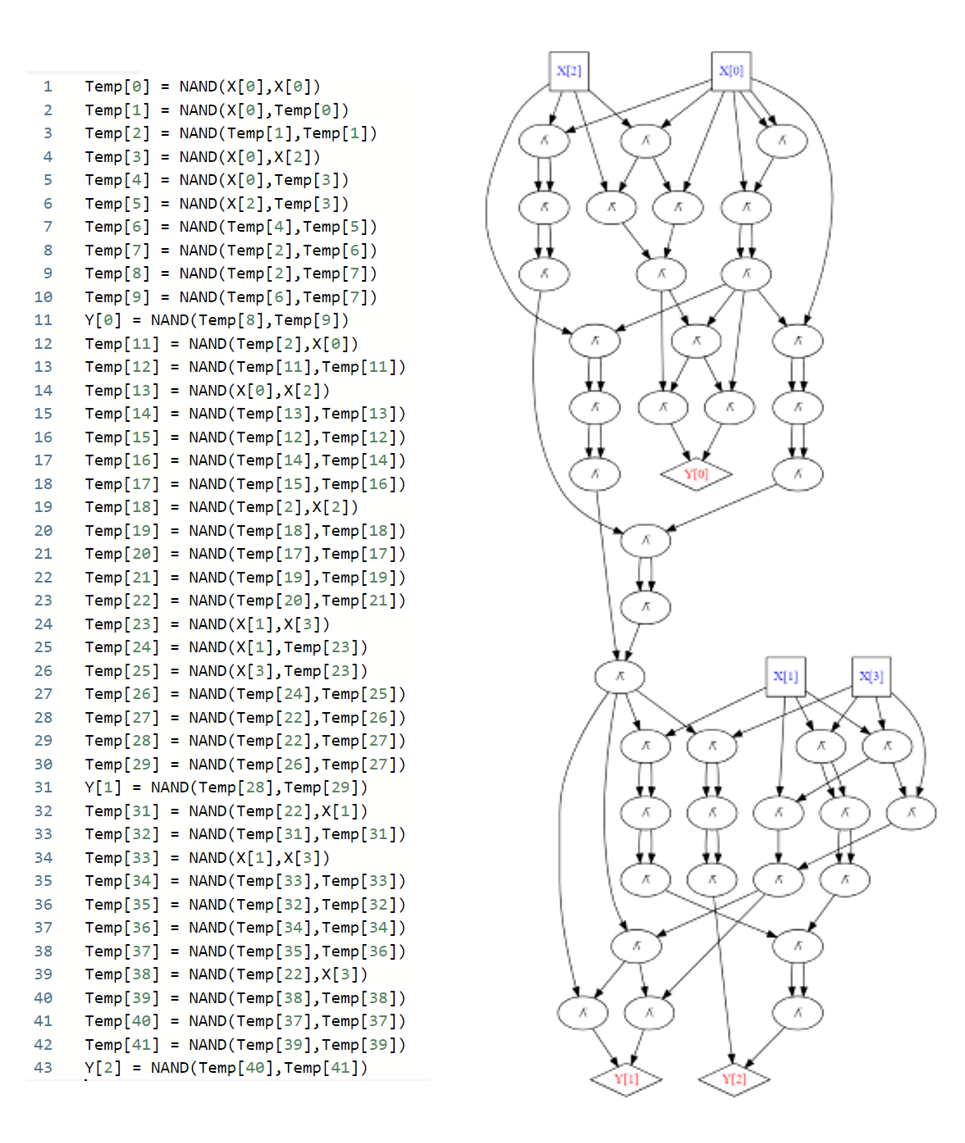
\includegraphics[width=\textwidth, height=0.25\paperheight, keepaspectratio]{../figure/add2bitnumbers.png}
\caption{The NAND-CIRC program and corresponding NAND circuit for adding
two-digit binary numbers that are obtained by ``expanding out'' all the
syntactic sugar. The program/circuit has 43 lines/gates which is by no
means necessary. It is possible to add \(n\) bit numbers using \(9n\)
NAND gates, see \cref{halffulladderex}.}
\label{add2bitnumbersfig}
\end{figure}

By going through the above program carefully and accounting for the
number of gates, we can see that it yields a proof of the following
theorem (see also \cref{addnumoflinesfig}):

\hypertarget{addition-thm}{}
\begin{theorem}[Addition using NAND-CIRC programs] \label[theorem]{addition-thm}

For every \(n\in \N\), let
\(\ensuremath{\mathit{ADD}}_n:\{0,1\}^{2n}\rightarrow \{0,1\}^{n+1}\) be
the function that, given \(x,x'\in \{0,1\}^n\) computes the
representation of the sum of the numbers that \(x\) and \(x'\)
represent. Then there is a constant \(c \leq 30\) such that for every
\(n\) there is a NAND-CIRC program of at most \(cn\) lines computing
\(\ensuremath{\mathit{ADD}}_n\).\footnote{The value of \(c\) can be
  improved to \(9\), see \cref{halffulladderex}.}

\end{theorem}


\begin{marginfigure}
\centering
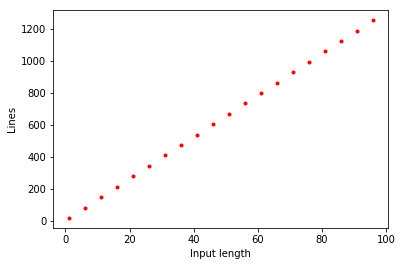
\includegraphics[width=\linewidth, height=1.5in, keepaspectratio]{../figure/addnumberoflines.png}
\caption{The number of lines in our NAND-CIRC program to add two \(n\)
bit numbers, as a function of \(n\), for \(n\)'s between \(1\) and
\(100\). This is not the most efficient program for this task, but the
important point is that it has the form \(O(n)\).}
\label{addnumoflinesfig}
\end{marginfigure}

Once we have addition, we can use the grade-school algorithm to obtain
multiplication as well, thus obtaining the following theorem:

\hypertarget{theoremid}{}
\begin{theorem}[Multiplication using NAND-CIRC programs] \label[theorem]{theoremid}

For every \(n\), let
\(\ensuremath{\mathit{MULT}}_n:\{0,1\}^{2n}\rightarrow \{0,1\}^{2n}\) be
the function that, given \(x,x'\in \{0,1\}^n\) computes the
representation of the product of the numbers that \(x\) and \(x'\)
represent. Then there is a constant \(c\) such that for every \(n\),
there is a NAND-CIRC program of at most \(cn^2\) that computes the
function \(\ensuremath{\mathit{MULT}}_n\).

\end{theorem}

We omit the proof, though in \cref{multiplication-ex} we ask you to
supply a ``constructive proof'' in the form of a program (in your
favorite programming language) that on input a number \(n\), outputs the
code of a NAND-CIRC program of at most \(1000n^2\) lines that computes
the \(\ensuremath{\mathit{MULT}}_n\) function. In fact, we can use
Karatsuba's algorithm to show that there is a NAND-CIRC program of
\(O(n^{\log_2 3})\) lines to compute \(\ensuremath{\mathit{MULT}}_n\)
(and can get even further asymptotic improvements using better
algorithms).

\section{The LOOKUP function}\label{seclookupfunc}

The \(\ensuremath{\mathit{LOOKUP}}\) function will play an important
role in this chapter and later. It is defined as follows:

\hypertarget{lookup-def}{}
\begin{definition}[Lookup function] \label[definition]{lookup-def}

For every \(k\), the \emph{lookup} function of order \(k\),
\(\ensuremath{\mathit{LOOKUP}}_k: \{0,1\}^{2^k+k}\rightarrow \{0,1\}\)
is defined as follows: For every \(x\in\{0,1\}^{2^k}\) and
\(i\in \{0,1\}^k\), \[
\ensuremath{\mathit{LOOKUP}}_k(x,i)=x_i
\] where \(x_i\) denotes the \(i^{th}\) entry of \(x\), using the binary
representation to identify \(i\) with a number in
\(\{0,\ldots,2^k - 1 \}\).

\end{definition}


\begin{figure}
\centering
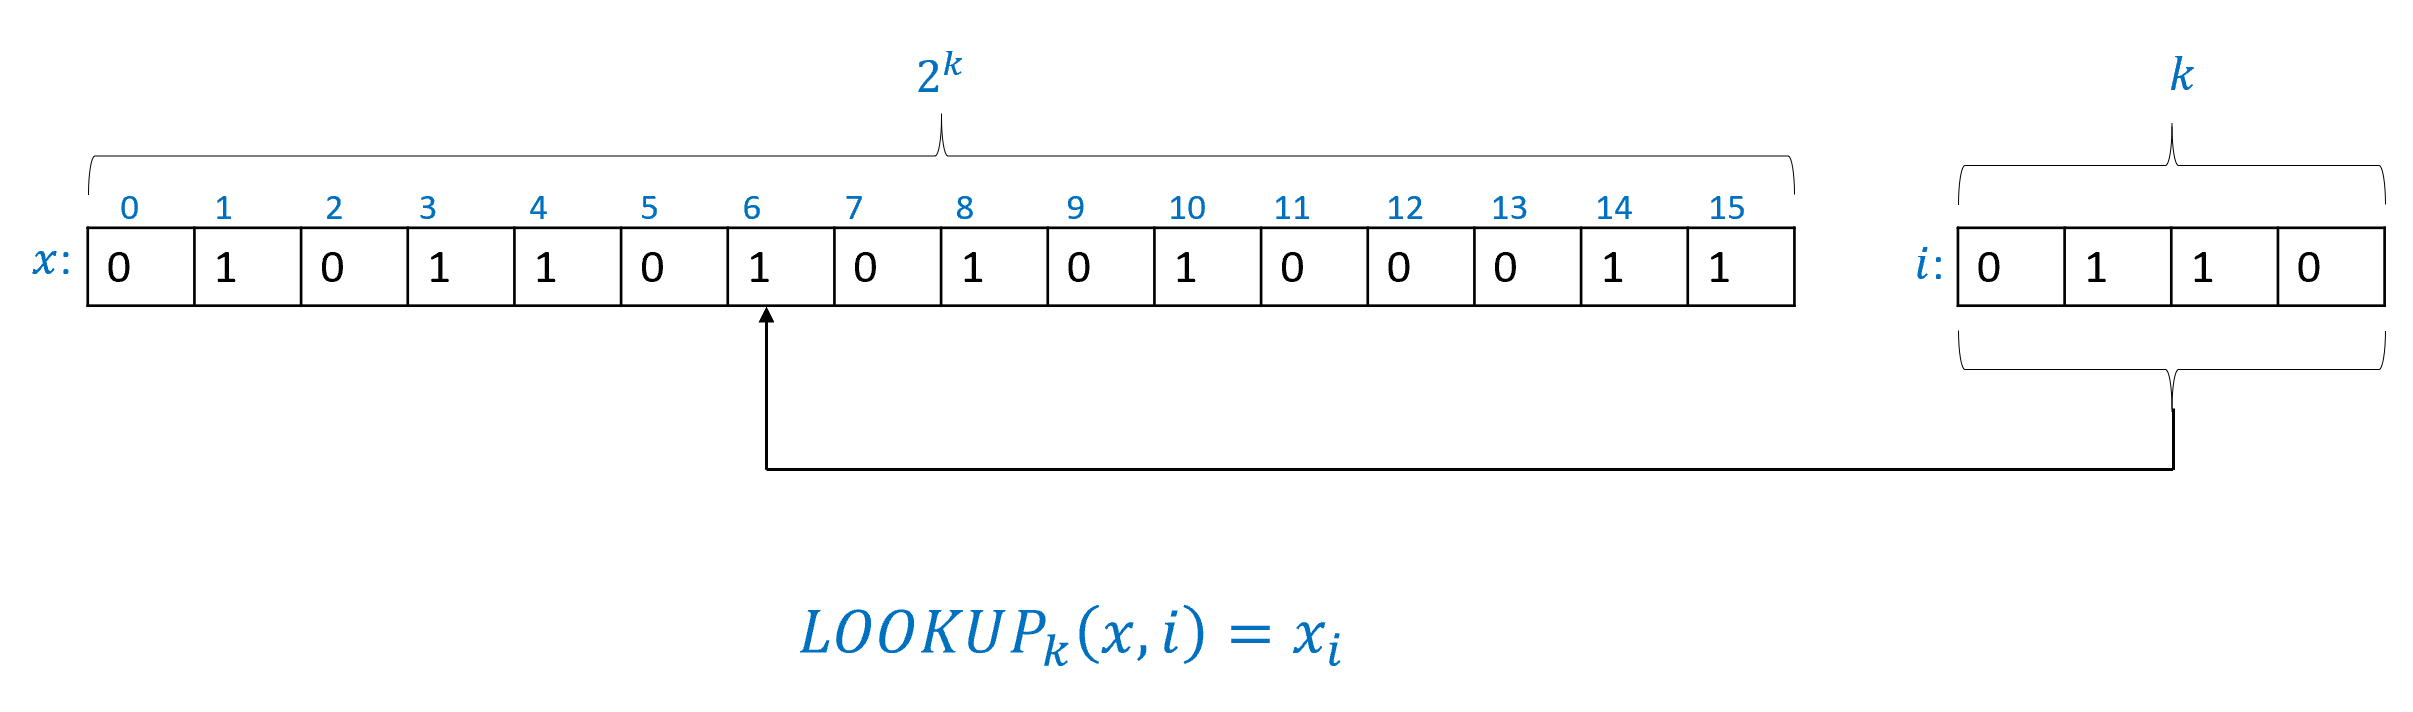
\includegraphics[width=\textwidth, height=0.25\paperheight, keepaspectratio]{../figure/lookupfunc.png}
\caption{The \(\ensuremath{\mathit{LOOKUP}}_k\) function takes an input
in \(\{0,1\}^{2^k+k}\), which we denote by \(x,i\) (with
\(x\in \{0,1\}^{2^k}\) and \(i \in \{0,1\}^k\)). The output is \(x_i\):
the \(i\)-th coordinate of \(x\), where we identify \(i\) as a number in
\([k]\) using the binary representation. In the above example
\(x\in \{0,1\}^{16}\) and \(i\in \{0,1\}^4\). Since \(i=0110\) is the
binary representation of the number \(6\), the output of
\(\ensuremath{\mathit{LOOKUP}}_4(x,i)\) in this case is \(x_6 = 1\).}
\label{lookupfig}
\end{figure}

See \cref{lookupfig} for an illustration of the LOOKUP function. It
turns out that for every \(k\), we can compute
\(\ensuremath{\mathit{LOOKUP}}_k\) using a NAND-CIRC program:

\hypertarget{lookup-thm}{}
\begin{theorem}[Lookup function] \label[theorem]{lookup-thm}

For every \(k>0\), there is a NAND-CIRC program that computes the
function
\(\ensuremath{\mathit{LOOKUP}}_k: \{0,1\}^{2^k+k}\rightarrow \{0,1\}\).
Moreover, the number of lines in this program is at most \(4\cdot 2^k\).

\end{theorem}

An immediate corollary of \cref{lookup-thm} is that for every \(k>0\),
\(\ensuremath{\mathit{LOOKUP}}_k\) can be computed by a Boolean circuit
(with AND, OR and NOT gates) of at most \(8 \cdot 2^k\) gates.

\subsection{Constructing a NAND-CIRC program for
\(\ensuremath{\mathit{LOOKUP}}\)}\label{Constructing-a-NAND-CIRC-}

We prove \cref{lookup-thm} by induction. For the case \(k=1\),
\(\ensuremath{\mathit{LOOKUP}}_1\) maps \((x_0,x_1,i) \in \{0,1\}^3\) to
\(x_i\). In other words, if \(i=0\) then it outputs \(x_0\) and
otherwise it outputs \(x_1\), which (up to reordering variables) is the
same as the \(\ensuremath{\mathit{IF}}\) function presented in
\cref{ifstatementsec}, which can be computed by a 4-line NAND-CIRC
program.

As a warm-up for the case of general \(k\), let us consider the case of
\(k=2\). Given input \(x=(x_0,x_1,x_2,x_3)\) for
\(\ensuremath{\mathit{LOOKUP}}_2\) and an index \(i=(i_0,i_1)\), if the
most significant bit \(i_0\) of the index is \(0\) then
\(\ensuremath{\mathit{LOOKUP}}_2(x,i)\) will equal \(x_0\) if \(i_1=0\)
and equal \(x_1\) if \(i_1=1\). Similarly, if the most significant bit
\(i_0\) is \(1\) then \(\ensuremath{\mathit{LOOKUP}}_2(x,i)\) will equal
\(x_2\) if \(i_1=0\) and will equal \(x_3\) if \(i_1=1\). Another way to
say this is that we can write \(\ensuremath{\mathit{LOOKUP}}_2\) as
follows:

\begin{code}
def LOOKUP2(X[0],X[1],X[2],X[3],i[0],i[1]):
    if i[0]==1:
        return LOOKUP1(X[2],X[3],i[1])
    else:
        return LOOKUP1(X[0],X[1],i[1])
\end{code}

or in other words,

\begin{code}
def LOOKUP2(X[0],X[1],X[2],X[3],i[0],i[1]):
    a = LOOKUP1(X[2],X[3],i[1])
    b = LOOKUP1(X[0],X[1],i[1])
    return IF( i[0],a,b)
\end{code}

More generally, as shown in the following lemma, we can compute
\(\ensuremath{\mathit{LOOKUP}}_k\) using two invocations of
\(\ensuremath{\mathit{LOOKUP}}_{k-1}\) and one invocation of
\(\ensuremath{\mathit{IF}}\):

\hypertarget{lookup-rec-lem}{}
\begin{lemma}[Lookup recursion] \label[lemma]{lookup-rec-lem}

For every \(k \geq 2\),
\(\ensuremath{\mathit{LOOKUP}}_k(x_0,\ldots,x_{2^k-1},i_0,\ldots,i_{k-1})\)
is equal to \[
\ensuremath{\mathit{IF}} \left(i_0, \ensuremath{\mathit{LOOKUP}}_{k-1}(x_{2^{k-1}},\ldots,x_{2^k-1},i_1,\ldots,i_{k-1}), \ensuremath{\mathit{LOOKUP}}_{k-1}(x_0,\ldots,x_{2^{k-1}-1},i_1,\ldots,i_{k-1}) \right)
\]

\end{lemma}

\begin{proof} \label[proof]{If-the-most-significant-b}

If the most significant bit \(i_{0}\) of \(i\) is zero, then the index
\(i\) is in \(\{0,\ldots,2^{k-1}-1\}\) and hence we can perform the
lookup on the ``first half'' of \(x\) and the result of
\(\ensuremath{\mathit{LOOKUP}}_k(x,i)\) will be the same as
\(a=\ensuremath{\mathit{LOOKUP}}_{k-1}(x_0,\ldots,x_{2^{k-1}-1},i_1,\ldots,i_{k-1})\).
On the other hand, if this most significant bit \(i_{0}\) is equal to
\(1\), then the index is in \(\{2^{k-1},\ldots,2^k-1\}\), in which case
the result of \(\ensuremath{\mathit{LOOKUP}}_k(x,i)\) is the same as
\(b=\ensuremath{\mathit{LOOKUP}}_{k-1}(x_{2^{k-1}},\ldots,x_{2^k-1},i_1,\ldots,i_{k-1})\).
Thus we can compute \(\ensuremath{\mathit{LOOKUP}}_k(x,i)\) by first
computing \(a\) and \(b\) and then outputting
\(\ensuremath{\mathit{IF}}(i_{k-1},a,b)\).

\end{proof}

\paragraph{Proof of \cref{lookup-thm} from \cref{lookup-rec-lem}.} Now
that we have \cref{lookup-rec-lem}, we can complete the proof of
\cref{lookup-thm}. We will prove by induction on \(k\) that there is a
NAND-CIRC program of at most \(4\cdot (2^k-1)\) lines for
\(\ensuremath{\mathit{LOOKUP}}_k\). For \(k=1\) this follows by the four
line program for \(\ensuremath{\mathit{IF}}\) we've seen before. For
\(k>1\), we use the following pseudocode:

\begin{code}
a = LOOKUP_(k-1)(X[0],...,X[2^(k-1)-1],i[1],...,i[k-1])
b = LOOKUP_(k-1)(X[2^(k-1)],...,Z[2^(k-1)],i[1],...,i[k-1])
return IF(i[0],b,a)
\end{code}

If we let \(L(k)\) be the number of lines required for
\(\ensuremath{\mathit{LOOKUP}}_k\), then the above pseudo-code shows
that \[
L(k) \leq 2L(k-1)+4 \;. \label{induction-lookup}
\] Since under our induction hypothesis \(L(k-1) \leq 4(2^{k-1}-1)\), we
get that \(L(k) \leq 2\cdot 4 (2^{k-1}-1) + 4 = 4(2^k - 1)\) which is
what we wanted to prove. See \cref{lookuplinesfig} for a plot of the
actual number of lines in our implementation of
\(\ensuremath{\mathit{LOOKUP}}_k\).


\begin{marginfigure}
\centering
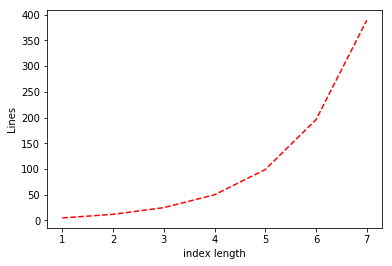
\includegraphics[width=\linewidth, height=1.5in, keepaspectratio]{../figure/lookup_numlines.png}
\caption{The number of lines in our implementation of the
\texttt{LOOKUP\_k} function as a function of \(k\) (i.e., the length of
the index). The number of lines in our implementation is roughly
\(3 \cdot 2^k\).}
\label{lookuplinesfig}
\end{marginfigure}

\section{Computing \emph{every} function}\label{seccomputeallfunctions}

At this point we know the following facts about NAND-CIRC programs (and
so equivalently about Boolean circuits and our other equivalent models):

\begin{enumerate}
\def\labelenumi{\arabic{enumi}.}
\item
  They can compute at least some non trivial functions.
\item
  Coming up with NAND-CIRC programs for various functions is a very
  tedious task.
\end{enumerate}

Thus I would not blame the reader if they were not particularly looking
forward to a long sequence of examples of functions that can be computed
by NAND-CIRC programs. However, it turns out we are not going to need
this, as we can show in one fell swoop that NAND-CIRC programs can
compute \emph{every} finite function:

\hypertarget{NAND-univ-thm}{}
\begin{theorem}[Universality of NAND] \label[theorem]{NAND-univ-thm}

There exists some constant \(c>0\) such that for every \(n,m>0\) and
function \(f: \{0,1\}^n\rightarrow \{0,1\}^m\), there is a NAND-CIRC
program with at most \(c \cdot m 2^n\) lines that computes the function
\(f\) .

\end{theorem}

By \cref{equivalencemodelsthm}, the models of NAND circuits, NAND-CIRC
programs, AON-CIRC programs, and Boolean circuits, are all equivalent to
one another, and hence \cref{NAND-univ-thm} holds for all these models.
In particular, the following theorem is equivalent to
\cref{NAND-univ-thm}:

\hypertarget{circuit-univ-thm}{}
\begin{theorem}[Universality of Boolean circuits] \label[theorem]{circuit-univ-thm}

There exists some constant \(c>0\) such that for every \(n,m>0\) and
function \(f: \{0,1\}^n\rightarrow \{0,1\}^m\), there is a Boolean
circuit with at most \(c \cdot m 2^n\) gates that computes the function
\(f\) .

\end{theorem}

\hypertarget{finitecomputation}{}
\begin{bigidea} \label[bigidea]{finitecomputation}

\emph{Every} finite function can be computed by a large enough Boolean
circuit.

\end{bigidea}

\emph{Improved bounds.} Though it will not be of great importance to us,
it is possible to improve on the proof of \cref{NAND-univ-thm} and shave
an extra factor of \(n\), as well as optimize the constant \(c\), and so
prove that for every \(\epsilon>0\), \(m\in \N\) and sufficiently large
\(n\), if \(f:\{0,1\}^n \rightarrow \{0,1\}^m\) then \(f\) can be
computed by a NAND circuit of at most
\((1+\epsilon)\tfrac{m\cdot 2^n}{n}\) gates. The proof of this result is
beyond the scope of this book, but we do discuss how to obtain a bound
of the form \(O(\tfrac{m \cdot 2^n}{n})\) in \cref{tight-upper-bound};
see also the biographical notes.

\subsection{Proof of NAND's
Universality}\label{Proof-of-NANDs-Universali}

To prove \cref{NAND-univ-thm}, we need to give a NAND circuit, or
equivalently a NAND-CIRC program, for \emph{every} possible function. We
will restrict our attention to the case of Boolean functions (i.e.,
\(m=1\)). \cref{mult-bit-ex} asks you to extend the proof for all values
of \(m\). A function \(F: \{0,1\}^n\rightarrow \{0,1\}\) can be
specified by a table of its values for each one of the \(2^n\) inputs.
For example, the table below describes one particular function
\(G: \{0,1\}^4 \rightarrow \{0,1\}\):\footnote{In case you are curious,
  this is the function on input \(i\in \{0,1\}^4\) (which we interpret
  as a number in \([16]\)), that outputs the \(i\)-th digit of \(\pi\)
  in the binary basis.}

\begin{longtable}[]{@{}ll@{}}
\caption{An example of a function \(G:\{0,1\}^4 \rightarrow \{0,1\}\).
\{ .table \#tablefunctiong \}}\tabularnewline
\toprule
Input (\(x\)) & Output (\(G(x)\))\tabularnewline
\midrule
\endfirsthead
\toprule
Input (\(x\)) & Output (\(G(x)\))\tabularnewline
\midrule
\endhead
\(0000\) & 1\tabularnewline
\(0001\) & 1\tabularnewline
\(0010\) & 0\tabularnewline
\(0011\) & 0\tabularnewline
\(0100\) & 1\tabularnewline
\(0101\) & 0\tabularnewline
\(0110\) & 0\tabularnewline
\(0111\) & 1\tabularnewline
\(1000\) & 0\tabularnewline
\(1001\) & 0\tabularnewline
\(1010\) & 0\tabularnewline
\(1011\) & 0\tabularnewline
\(1100\) & 1\tabularnewline
\(1101\) & 1\tabularnewline
\(1110\) & 1\tabularnewline
\(1111\) & 1\tabularnewline
\bottomrule
\end{longtable}

For every \(x\in \{0,1\}^4\),
\(G(x)=\ensuremath{\mathit{LOOKUP}}_4(1100100100001111,x)\), and so the
following is NAND-CIRC ``pseudocode'' to compute \(G\) using syntactic
sugar for the \texttt{LOOKUP\_4} procedure.

\begin{code}
G0000 = 1
G1000 = 1
G0100 = 0
...
G0111 = 1
G1111 = 1
Y[0] = LOOKUP_4(G0000,G1000,...,G1111,
                X[0],X[1],X[2],X[3])
\end{code}

We can translate this pseudocode into an actual NAND-CIRC program by
adding three lines to define variables \texttt{zero} and \texttt{one}
that are initialized to \(0\) and \(1\) respectively, and then replacing
a statement such as \texttt{Gxxx = 0} with \texttt{Gxxx = NAND(one,one)}
and a statement such as \texttt{Gxxx = 1} with
\texttt{Gxxx = NAND(zero,zero)}. The call to \texttt{LOOKUP\_4} will be
replaced by the NAND-CIRC program that computes
\(\ensuremath{\mathit{LOOKUP}}_4\), plugging in the appropriate inputs.

There was nothing about the above reasoning that was particular to the
function \(G\) of \cref{tablefunctiong}. Given \emph{every} function
\(F: \{0,1\}^n \rightarrow \{0,1\}\), we can write a NAND-CIRC program
that does the following:

\begin{enumerate}
\def\labelenumi{\arabic{enumi}.}
\item
  Initialize \(2^n\) variables of the form \texttt{F00...0} till
  \texttt{F11...1} so that for every \(z\in\{0,1\}^n\), the variable
  corresponding to \(z\) is assigned the value \(F(z)\).
\item
  Compute \(\ensuremath{\mathit{LOOKUP}}_n\) on the \(2^n\) variables
  initialized in the previous step, with the index variable being the
  input variables \texttt{X[}\(0\)
  \texttt{]},\ldots,\texttt{X[}\(2^n-1\) \texttt{]}. That is, just like
  in the pseudocode for \texttt{G} above, we use
  \texttt{Y[0] = LOOKUP(F00..00,...,F11..1,X[0],..,x[}\(n-1\)\texttt{])}
\end{enumerate}

The total number of lines in the resulting program is \(3+2^n\) lines
for initializing the variables plus the \(4\cdot 2^n\) lines that we pay
for computing \(\ensuremath{\mathit{LOOKUP}}_n\). This completes the
proof of \cref{NAND-univ-thm}.

\hypertarget{discusscomputation}{}
\begin{remark}[Result in perspective] \label[remark]{discusscomputation}

While \cref{NAND-univ-thm} seems striking at first, in retrospect, it is
perhaps not that surprising that every finite function can be computed
with a NAND-CIRC program. After all, a finite function
\(F: \{0,1\}^n \rightarrow \{0,1\}^m\) can be represented by simply the
list of its outputs for each one of the \(2^n\) input values. So it
makes sense that we could write a NAND-CIRC program of similar size to
compute it. What is more interesting is that \emph{some} functions, such
as addition and multiplication, have a much more efficient
representation: one that only requires \(O(n^2)\) or even fewer lines.

\end{remark}

\subsection{Improving by a factor of \(n\)
(optional)}\label{tight-upper-bound}

By being a little more careful, we can improve the bound of
\cref{NAND-univ-thm} and show that every function
\(F:\{0,1\}^n \rightarrow \{0,1\}^m\) can be computed by a NAND-CIRC
program of at most \(O(m 2^n/n)\) lines. In other words, we can prove
the following improved version:

\hypertarget{NAND-univ-thm-improved}{}
\begin{theorem}[Universality of NAND circuits, improved bound] \label[theorem]{NAND-univ-thm-improved}

There exists a constant \(c>0\) such that for every \(n,m>0\) and
function \(f: \{0,1\}^n\rightarrow \{0,1\}^m\), there is a NAND-CIRC
program with at most \(c \cdot m 2^n / n\) lines that computes the
function \(f\).\footnote{The constant \(c\) in this theorem is at most
  \(10\) and in fact can be arbitrarily close to \(1\), see
  \cref{computeeveryfunctionbibnotes}.}

\end{theorem}

\begin{proof} \label[proof]{As-before-it-is-enough-to}

As before, it is enough to prove the case that \(m=1\). Hence we let
\(f:\{0,1\}^n \rightarrow \{0,1\}\), and our goal is to prove that there
exists a NAND-CIRC program of \(O(2^n/n)\) lines (or equivalently a
Boolean circuit of \(O(2^n/n)\) gates) that computes \(f\).

We let \(k= \log(n-2\log n)\) (the reasoning behind this choice will
become clear later on). We define the function
\(g:\{0,1\}^k \rightarrow \{0,1\}^{2^{n-k}}\) as follows: \[
g(a) = f(a0^{n-k})f(a0^{n-k-1}1) \cdots f(a1^{n-k}) \;.
\] In other words, if we use the usual binary representation to identify
the numbers \(\{0,\ldots, 2^{n-k}-1 \}\) with the strings
\(\{0,1\}^{n-k}\), then for every \(a\in \{0,1\}^k\) and
\(b\in \{0,1\}^{n-k}\) \[
g(a)_b = f(ab) \;. \label{eqcomputefusinggeffcircuit}
\]


\begin{marginfigure}
\centering
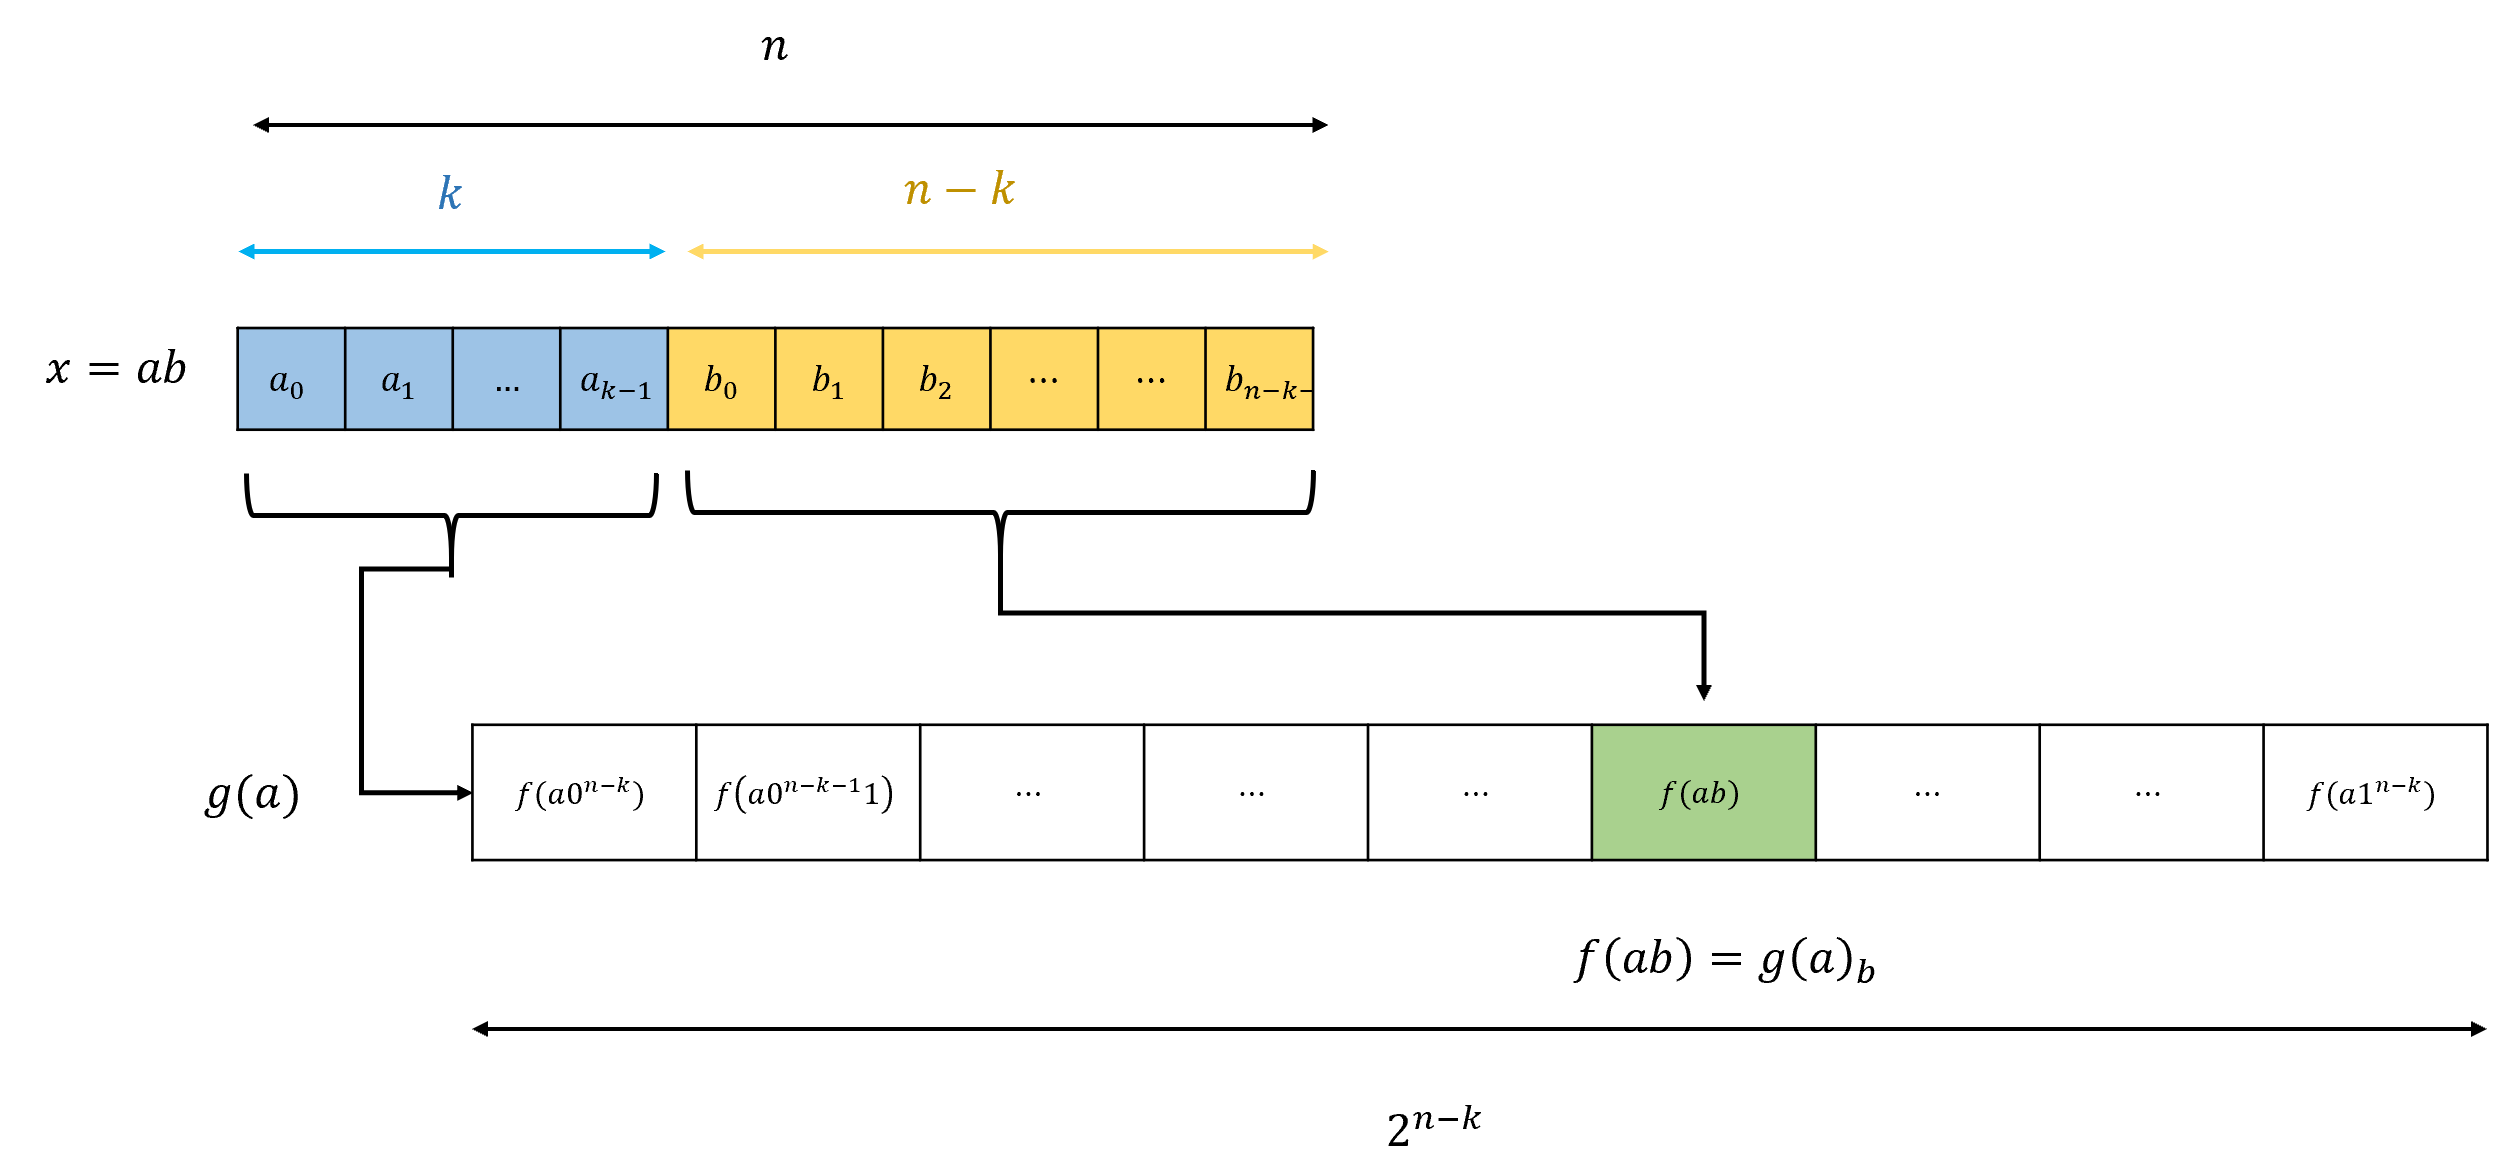
\includegraphics[width=\linewidth, height=1.5in, keepaspectratio]{../figure/efficient_circuit_allfunc.png}
\caption{We can compute \(f:\{0,1\}^n \rightarrow \{0,1\}\) on input
\(x=ab\) where \(a\in \{0,1\}^k\) and \(b\in \{0,1\}^{n-k}\) by first
computing the \(2^{n-k}\) long string \(g(a)\) that corresponds to all
\(f\)'s values on inputs that begin with \(a\), and then outputting the
\(b\)-th coordinate of this string.}
\label{efficient_circuit_allfuncfig}
\end{marginfigure}

\eqref{eqcomputefusinggeffcircuit} means that for every
\(x\in \{0,1\}^n\), if we write \(x=ab\) with \(a\in \{0,1\}^k\) and
\(b\in \{0,1\}^{n-k}\) then we can compute \(f(x)\) by first computing
the string \(T=g(a)\) of length \(2^{n-k}\), and then computing
\(\ensuremath{\mathit{LOOKUP}}_{n-k}(T\;,\; b)\) to retrieve the element
of \(T\) at the position corresponding to \(b\) (see
\cref{efficient_circuit_allfuncfig}). The cost to compute the
\(\ensuremath{\mathit{LOOKUP}}_{n-k}\) is \(O(2^{n-k})\) lines/gates and
the cost in NAND-CIRC lines (or Boolean gates) to compute \(f\) is at
most \[
cost(g) + O(2^{n-k}) \;, \label{eqcostcomputefusingg}
\] where \(cost(g)\) is the number of operations (i.e., lines of
NAND-CIRC programs or gates in a circuit) needed to compute \(g\).

To complete the proof we need to give a bound on \(cost(g)\). Since
\(g\) is a function mapping \(\{0,1\}^k\) to \(\{0,1\}^{2^{n-k}}\), we
can also think of it as a collection of \(2^{n-k}\) functions
\(g_0,\ldots, g_{2^{n-k}-1}: \{0,1\}^k \rightarrow \{0,1\}\), where
\(g_i(x) = g(a)_i\) for every \(a\in \{0,1\}^k\) and \(i\in [2^{n-k}]\).
(That is, \(g_i(a)\) is the \(i\)-th bit of \(g(a)\).) Naively, we could
use \cref{NAND-univ-thm} to compute each \(g_i\) in \(O(2^k)\) lines,
but then the total cost is \(O(2^{n-k} \cdot 2^k) = O(2^n)\) which does
not save us anything. However, the crucial observation is that there are
only \(2^{2^k}\) \emph{distinct functions} mapping \(\{0,1\}^k\) to
\(\{0,1\}\). For example, if \(g_{17}\) is an identical function to
\(g_{67}\) that means that if we already computed \(g_{17}(a)\) then we
can compute \(g_{67}(a)\) using only a constant number of operations:
simply copy the same value! In general, if you have a collection of
\(N\) functions \(g_0,\ldots,g_{N-1}\) mapping \(\{0,1\}^k\) to
\(\{0,1\}\), of which at most \(S\) are distinct then for every value
\(a\in \{0,1\}^k\) we can compute the \(N\) values
\(g_0(a),\ldots,g_{N-1}(a)\) using at most \(O(S\cdot 2^k + N)\)
operations (see \cref{computemanyfunctionsfig}).


\begin{marginfigure}
\centering
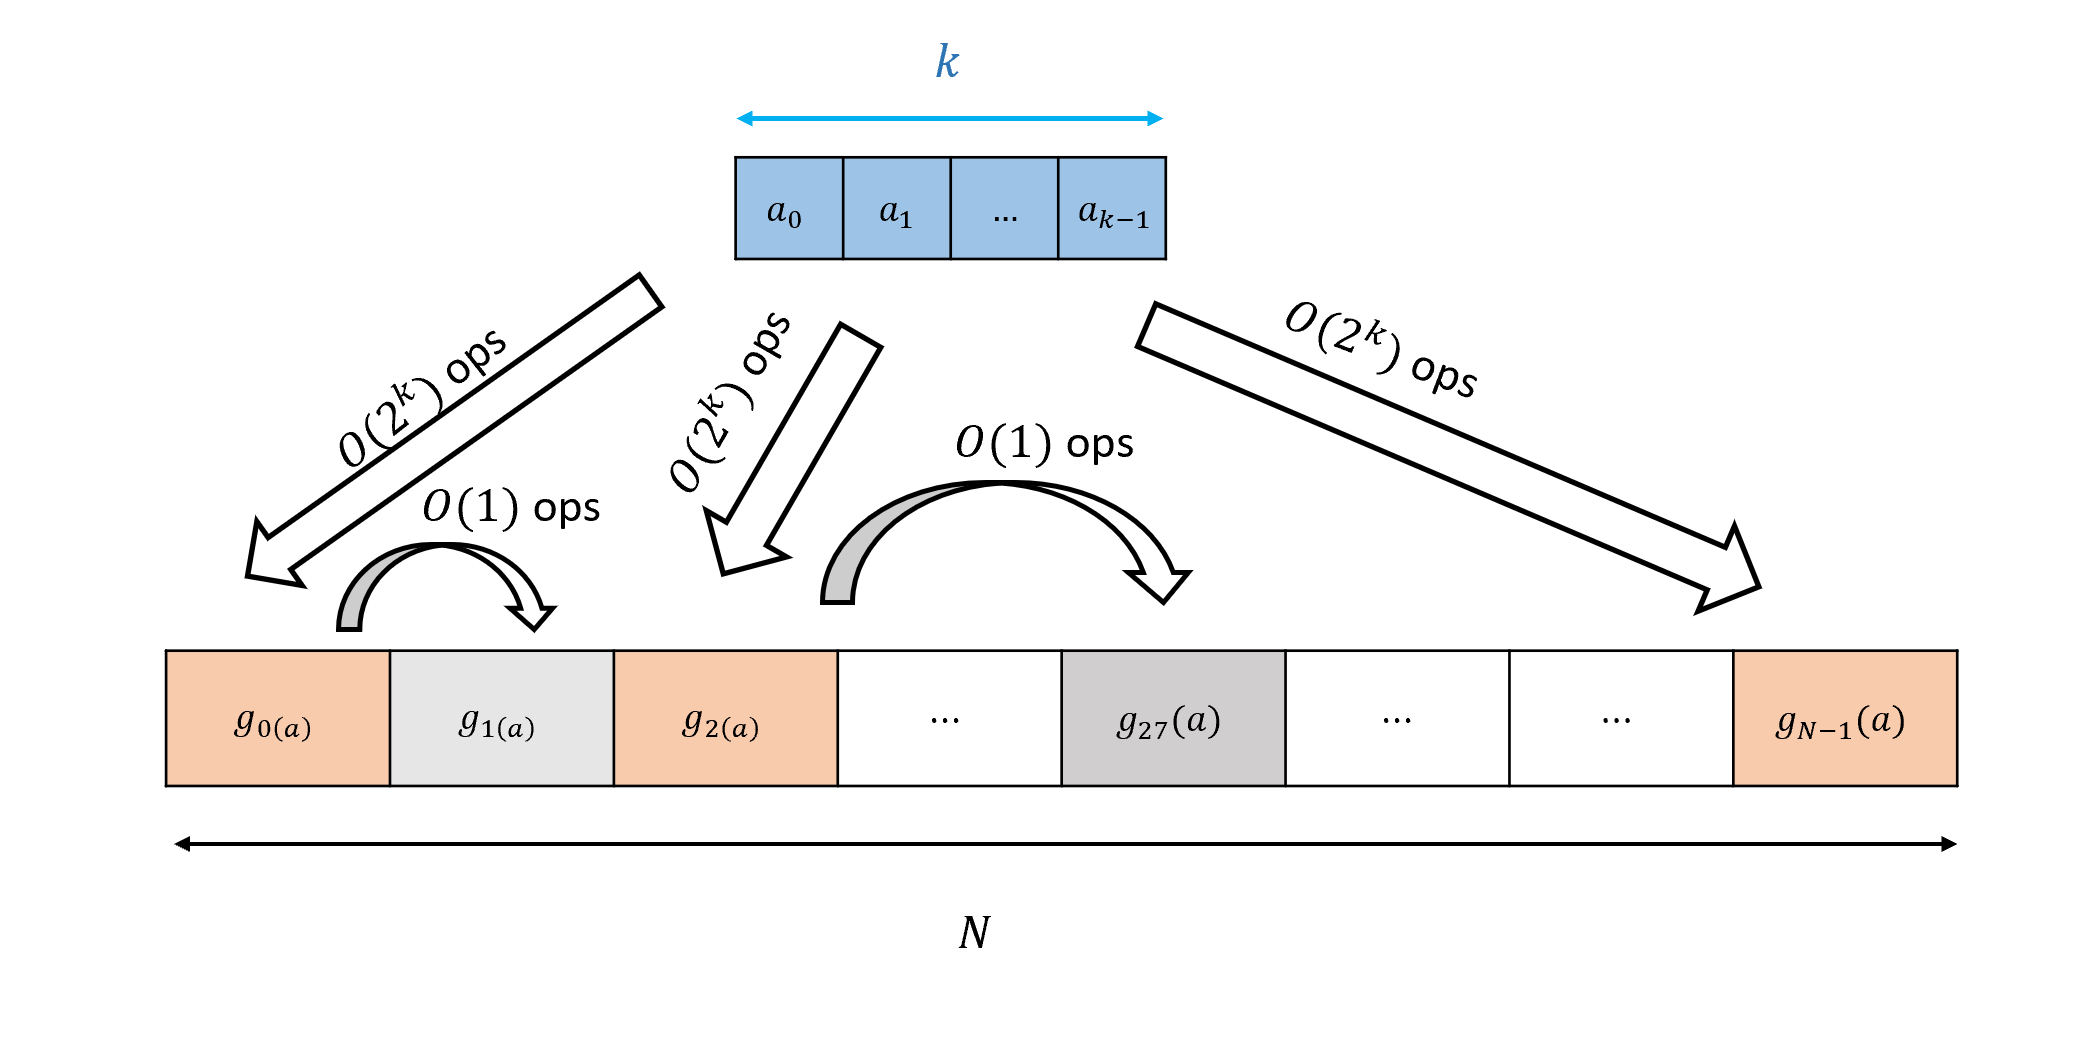
\includegraphics[width=\linewidth, height=1.5in, keepaspectratio]{../figure/computemanyfunctions.png}
\caption{If \(g_0,\ldots, g_{N-1}\) is a collection of functions each
mapping \(\{0,1\}^k\) to \(\{0,1\}\) such that at most \(S\) of them are
distinct then for every \(a\in \{0,1\}^k\), we can compute all the
values \(g_0(a),\ldots,g_{N-1}(a)\) using at most \(O(S \cdot 2^k + N)\)
operations by first computing the distinct functions and then copying
the resulting values.}
\label{computemanyfunctionsfig}
\end{marginfigure}

In our case, because there are at most \(2^{2^k}\) distinct functions
mapping \(\{0,1\}^k\) to \(\{0,1\}\), we can compute the function \(g\)
(and hence by \eqref{eqcomputefusinggeffcircuit} also \(f\)) using at
most\\
\[O(2^{2^k} \cdot 2^k + 2^{n-k}) \label{eqboundoncostg}\] operations.
Now all that is left is to plug into \eqref{eqboundoncostg} our choice
of \(k = \log (n-2\log n)\). By definition, \(2^k = n-2\log n\), which
means that \eqref{eqboundoncostg} can be bounded \[
O\left(2^{n-2\log n} \cdot (n-2\log n) +  2^{n-\log(n-2\log n)}\right) \leq
\]

\[
O\left(\tfrac{2^n}{n^2} \cdot n + \tfrac{2^n}{n-2\log n} \right)
\leq
O\left(\tfrac{2^n}{n}  + \tfrac{2^n}{0.5n} \right)  = O\left( \tfrac{2^n}{n} \right)
\] which is what we wanted to prove. (We used above the fact that
\(n - 2\log n \geq 0.5 \log n\) for sufficiently large \(n\).)

\end{proof}

Using the connection between NAND-CIRC programs and Boolean circuits, an
immediate corollary of \cref{NAND-univ-thm-improved} is the following
improvement to \cref{circuit-univ-thm}:

\hypertarget{circuit-univ-thm-improved}{}
\begin{theorem}[Universality of Boolean circuits,  improved bound] \label[theorem]{circuit-univ-thm-improved}

There exists some constant \(c>0\) such that for every \(n,m>0\) and
function \(f: \{0,1\}^n\rightarrow \{0,1\}^m\), there is a Boolean
circuit with at most \(c \cdot m 2^n / n\) gates that computes the
function \(f\) .

\end{theorem}

\section{Computing every function: An alternative
proof}\label{seccomputalternative}

\cref{circuit-univ-thm} is a fundamental result in the theory (and
practice!) of computation. In this section we present an alternative
proof of this basic fact that Boolean circuits can compute every finite
function. This alternative proof gives a somewhat worse quantitative
bound on the number of gates but it has the advantage of being simpler,
working directly with circuits and avoiding the usage of all the
syntactic sugar machinery. (However, that machinery is useful in its own
right, and will find other applications later on.)

\hypertarget{circuit-univ-alt-thm}{}
\begin{theorem}[Universality of Boolean circuits (alternative phrasing)] \label[theorem]{circuit-univ-alt-thm}

There exists some constant \(c>0\) such that for every \(n,m>0\) and
function \(f: \{0,1\}^n\rightarrow \{0,1\}^m\), there is a Boolean
circuit with at most \(c \cdot m\cdot n 2^n\) gates that computes the
function \(f\) .

\end{theorem}


\begin{figure}
\centering
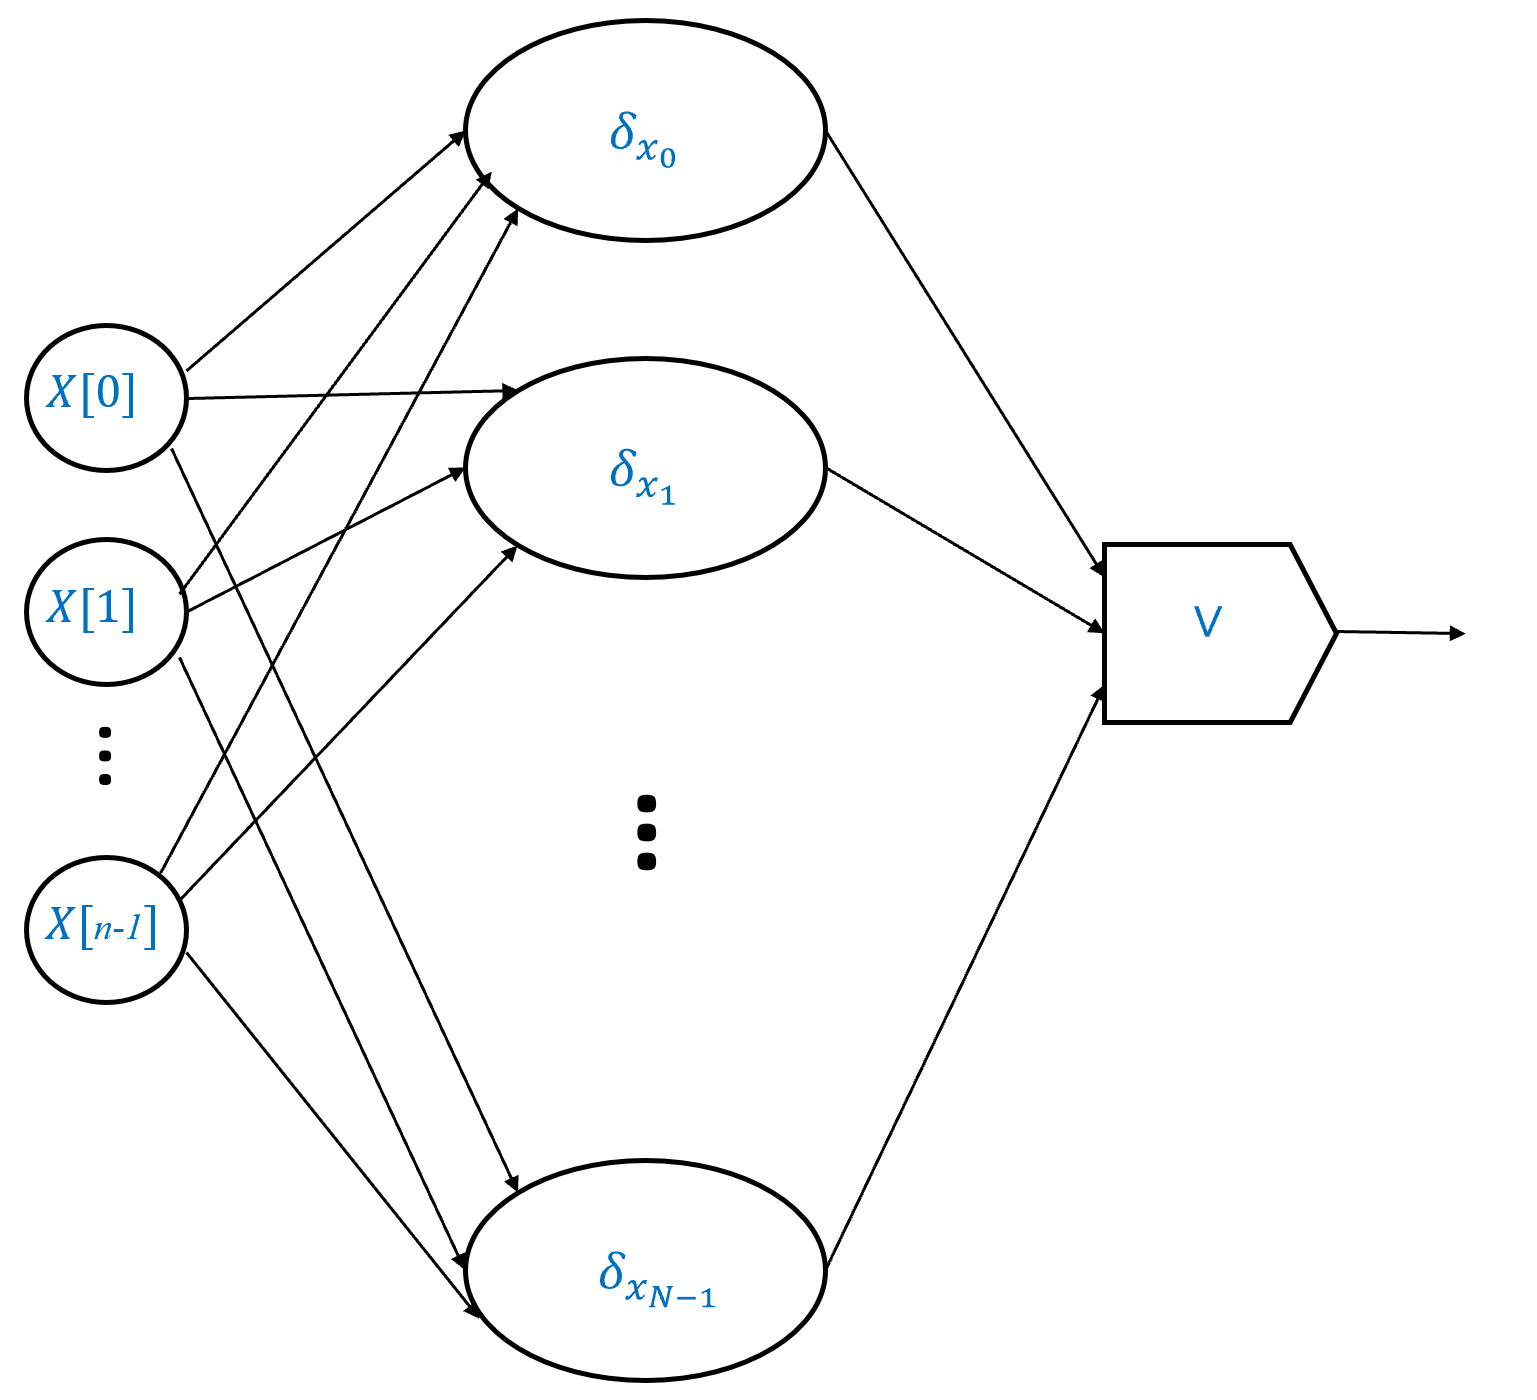
\includegraphics[width=\textwidth, height=0.25\paperheight, keepaspectratio]{../figure/computeallfunctionalt.png}
\caption{Given a function \(f:\{0,1\}^n \rightarrow \{0,1\}\), we let
\(\{ x_0, x_1, \ldots, x_{N-1} \} \subseteq \{0,1\}^n\) be the set of
inputs such that \(f(x_i)=1\), and note that \(N \leq 2^n\). We can
express \(f\) as the OR of \(\delta_{x_i}\) for \(i\in [N]\) where the
function \(\delta_\alpha:\{0,1\}^n \rightarrow \{0,1\}\) (for
\(\alpha \in \{0,1\}^n\)) is defined as follows: \(\delta_\alpha(x)=1\)
iff \(x=\alpha\). We can compute the OR of \(N\) values using \(N\)
two-input OR gates. Therefore if we have a circuit of size \(O(n)\) to
compute \(\delta_\alpha\) for every \(\alpha \in \{0,1\}^n\), we can
compute \(f\) using a circuit of size
\(O(n \cdot N) = O(n \cdot 2^n)\).}
\label{computeallfuncaltfig}
\end{figure}

\begin{proofidea} \label[proofidea]{The-idea-of-the-proof-is-}

The idea of the proof is illustrated in \cref{computeallfuncaltfig}. As
before, it is enough to focus on the case that \(m=1\) (the function
\(f\) has a single output), since we can always extend this to the case
of \(m>1\) by looking at the composition of \(m\) circuits each
computing a different output bit of the function \(f\). We start by
showing that for every \(\alpha \in \{0,1\}^n\), there is an \(O(n)\)
sized circuit that computes the function
\(\delta_\alpha:\{0,1\}^n \rightarrow \{0,1\}\) defined as follows:
\(\delta_\alpha(x)=1\) iff \(x=\alpha\) (that is, \(\delta_\alpha\)
outputs \(0\) on all inputs except the input \(\alpha\)). We can then
write any function \(f:\{0,1\}^n \rightarrow \{0,1\}\) as the OR of at
most \(2^n\) functions \(\delta_\alpha\) for the \(\alpha\)'s on which
\(f(\alpha)=1\).

\end{proofidea}

\begin{proof}[Proof of \cref{circuit-univ-alt-thm}] \label[proof]{We-prove-the-theorem-for-}

We prove the theorem for the case \(m=1\). The result can be extended
for \(m>1\) as before (see also \cref{mult-bit-ex}). Let
\(f:\{0,1\}^n \rightarrow \{0,1\}\). We will prove that there is an
\(O(n\cdot 2^n)\)-sized Boolean circuit to compute \(f\) in the
following steps:

\begin{enumerate}
\def\labelenumi{\arabic{enumi}.}
\item
  We show that for every \(\alpha\in \{0,1\}^n\), there is an \(O(n)\)
  sized circuit that computes the function
  \(\delta_\alpha:\{0,1\}^n \rightarrow \{0,1\}\), where
  \(\delta_\alpha(x)=1\) iff \(x=\alpha\).
\item
  We then show that this implies the existence of an
  \(O(n\cdot 2^n)\)-sized circuit that computes \(f\), by writing
  \(f(x)\) as the OR of \(\delta_\alpha(x)\) for all
  \(\alpha\in \{0,1\}^n\) such that \(f(\alpha)=1\).
\end{enumerate}

We start with Step 1:

\textbf{CLAIM:} For \(\alpha \in \{0,1\}^n\), define
\(\delta_\alpha:\{0,1\}^n\) as follows: \[
\delta_\alpha(x) = \begin{cases}1 & x=\alpha \\ 0 & \text{otherwise} \end{cases} \;.
\] then there is a Boolean circuit using at most \(2n\) gates that
computes \(\delta_\alpha\).

\textbf{PROOF OF CLAIM:} The proof is illustrated in
\cref{deltafuncfig}. As an example, consider the function
\(\delta_{011}:\{0,1\}^3 \rightarrow \{0,1\}\). This function outputs
\(1\) on \(x\) if and only if \(x_0=0\), \(x_1=1\) and \(x_2=1\), and so
we can write \(\delta_{011}(x) = \overline{x_0} \wedge x_1 \wedge x_2\),
which translates into a Boolean circuit with one NOT gate and two AND
gates. More generally, for every \(\alpha \in \{0,1\}^n\), we can
express \(\delta_{\alpha}(x)\) as
\((x_0 = \alpha_0) \wedge (x_1 = \alpha_1) \wedge \cdots \wedge (x_{n-1} = \alpha_{n-1})\),
where if \(\alpha_i=0\) we replace \(x_i = \alpha_i\) with
\(\overline{x_i}\) and if \(\alpha_i=1\) we replace \(x_i=\alpha_i\) by
simply \(x_i\). This yields a circuit that computes \(\delta_\alpha\)
using \(n\) AND gates and at most \(n\) NOT gates, so a total of at most
\(2n\) gates.

Now for every function \(f:\{0,1\}^n \rightarrow \{0,1\}\), we can write

\[
f(x) = \delta_{x_0}(x) \vee \delta_{x_1}(x) \vee \cdots \vee \delta_{x_{N-1}}(x) \label{eqorofdeltafunc}
\]

where \(S=\{ x_0 ,\ldots, x_{N-1}\}\) is the set of inputs on which
\(f\) outputs \(1\). (To see this, you can verify that the right-hand
side of \eqref{eqorofdeltafunc} evaluates to \(1\) on \(x\in \{0,1\}^n\)
if and only if \(x\) is in the set \(S\).)

Therefore we can compute \(f\) using a Boolean circuit of at most \(2n\)
gates for each of the \(N\) functions \(\delta_{x_i}\) and combine that
with at most \(N\) OR gates, thus obtaining a circuit of at most
\(2n\cdot N + N\) gates. Since \(S \subseteq \{0,1\}^n\), its size \(N\)
is at most \(2^n\) and hence the total number of gates in this circuit
is \(O(n\cdot 2^n)\).

\end{proof}


\begin{marginfigure}
\centering
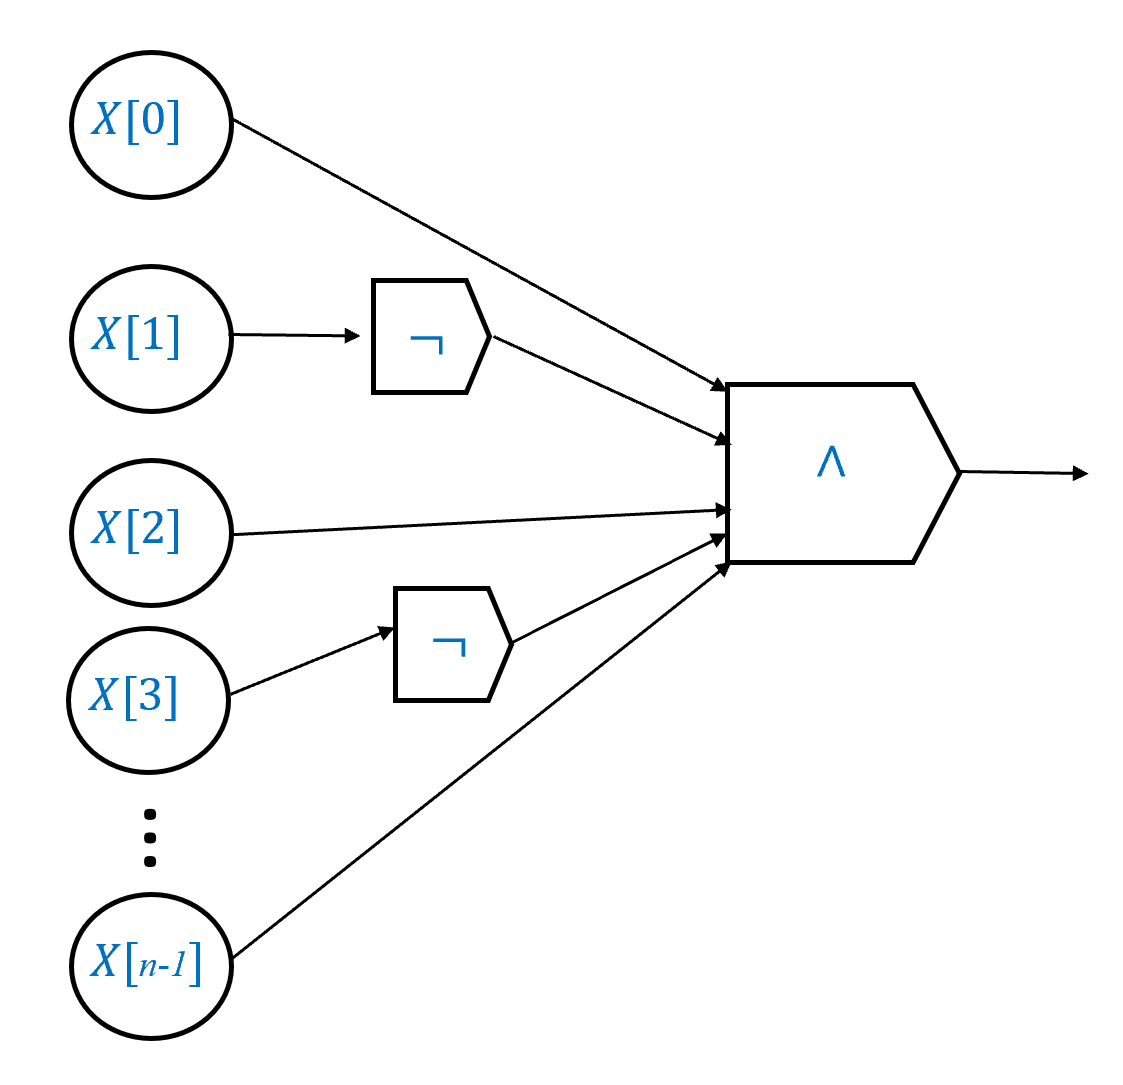
\includegraphics[width=\linewidth, height=1.5in, keepaspectratio]{../figure/deltafunc.png}
\caption{For every string \(\alpha\in \{0,1\}^n\), there is a Boolean
circuit of \(O(n)\) gates to compute the function
\(\delta_\alpha:\{0,1\}^n \rightarrow \{0,1\}\) such that
\(\delta_\alpha(x)=1\) if and only if \(x=\alpha\). The circuit is very
simple. Given input \(x_0,\ldots,x_{n-1}\) we compute the AND of
\(z_0,\ldots,z_{n-1}\) where \(z_i=x_i\) if \(\alpha_i=1\) and
\(z_i = \ensuremath{\mathit{NOT}}(x_i)\) if \(\alpha_i=0\). While
formally Boolean circuits only have a gate for computing the AND of two
inputs, we can implement an AND of \(n\) inputs by composing \(n\)
two-input ANDs.}
\label{deltafuncfig}
\end{marginfigure}

\section{The class
\(\ensuremath{\mathit{SIZE}}(T)\)}\label{secdefinesizeclasses}

We have seen that \emph{every} function
\(f:\{0,1\}^n \rightarrow \{0,1\}^m\) can be computed by a circuit of
size \(O(m\cdot 2^n)\), and \emph{some} functions (such as addition and
multiplication) can be computed by much smaller circuits. We define
\(\ensuremath{\mathit{SIZE}}(s)\) to be the set of functions that can be
computed by NAND circuits of at most \(s\) gates (or equivalently, by
NAND-CIRC programs of at most \(s\) lines). Formally, the definition is
as follows:

\hypertarget{sizedef}{}
\begin{definition}[Size class of functions] \label[definition]{sizedef}

For every \(n,m \in \{ 1, \ldots , 2s\}\), we let set
\(\ensuremath{\mathit{SIZE}}_{n,m}(s)\) denotes the set of all functions
\(f:\{0,1\}^n \rightarrow \{0,1\}^m\) such that
\(f\in \ensuremath{\mathit{SIZE}}(s)\).\footnote{The restriction that
  \(m,n \leq 2s\) makes no difference; see \cref{nandcircsizeex}.} We
denote by \(\ensuremath{\mathit{SIZE}}_n(s)\) the set
\(\ensuremath{\mathit{SIZE}}_{n,1}(s)\). For every integer \(s \geq 1\),
we let
\(\ensuremath{\mathit{SIZE}}(s) = \cup_{n,m \leq 2s} \ensuremath{\mathit{SIZE}}_{n,m}(s)\)
be the set of all functions \(f\) for which there exists a NAND circuit
of at most \(s\) gates that compute \(f\).

\end{definition}

\cref{funcvscircfig} depicts the sets
\(\ensuremath{\mathit{SIZE}}_{n,1}(s)\). Note that
\(\ensuremath{\mathit{SIZE}}_{n,m}(s)\) is a set of \emph{functions},
not of \emph{programs!} (asking if a program or a circuit is a member of
\(\ensuremath{\mathit{SIZE}}_{n,m}(s)\) is a \emph{category error} as in
the sense of \cref{cucumberfig}). As we discussed in
\cref{specvsimplrem} (and \cref{secimplvsspec}), the distinction between
\emph{programs} and \emph{functions} is absolutely crucial. You should
always remember that while a program \emph{computes} a function, it is
not \emph{equal} to a function. In particular, as we've seen, there can
be more than one program to compute the same function.


\begin{figure}
\centering
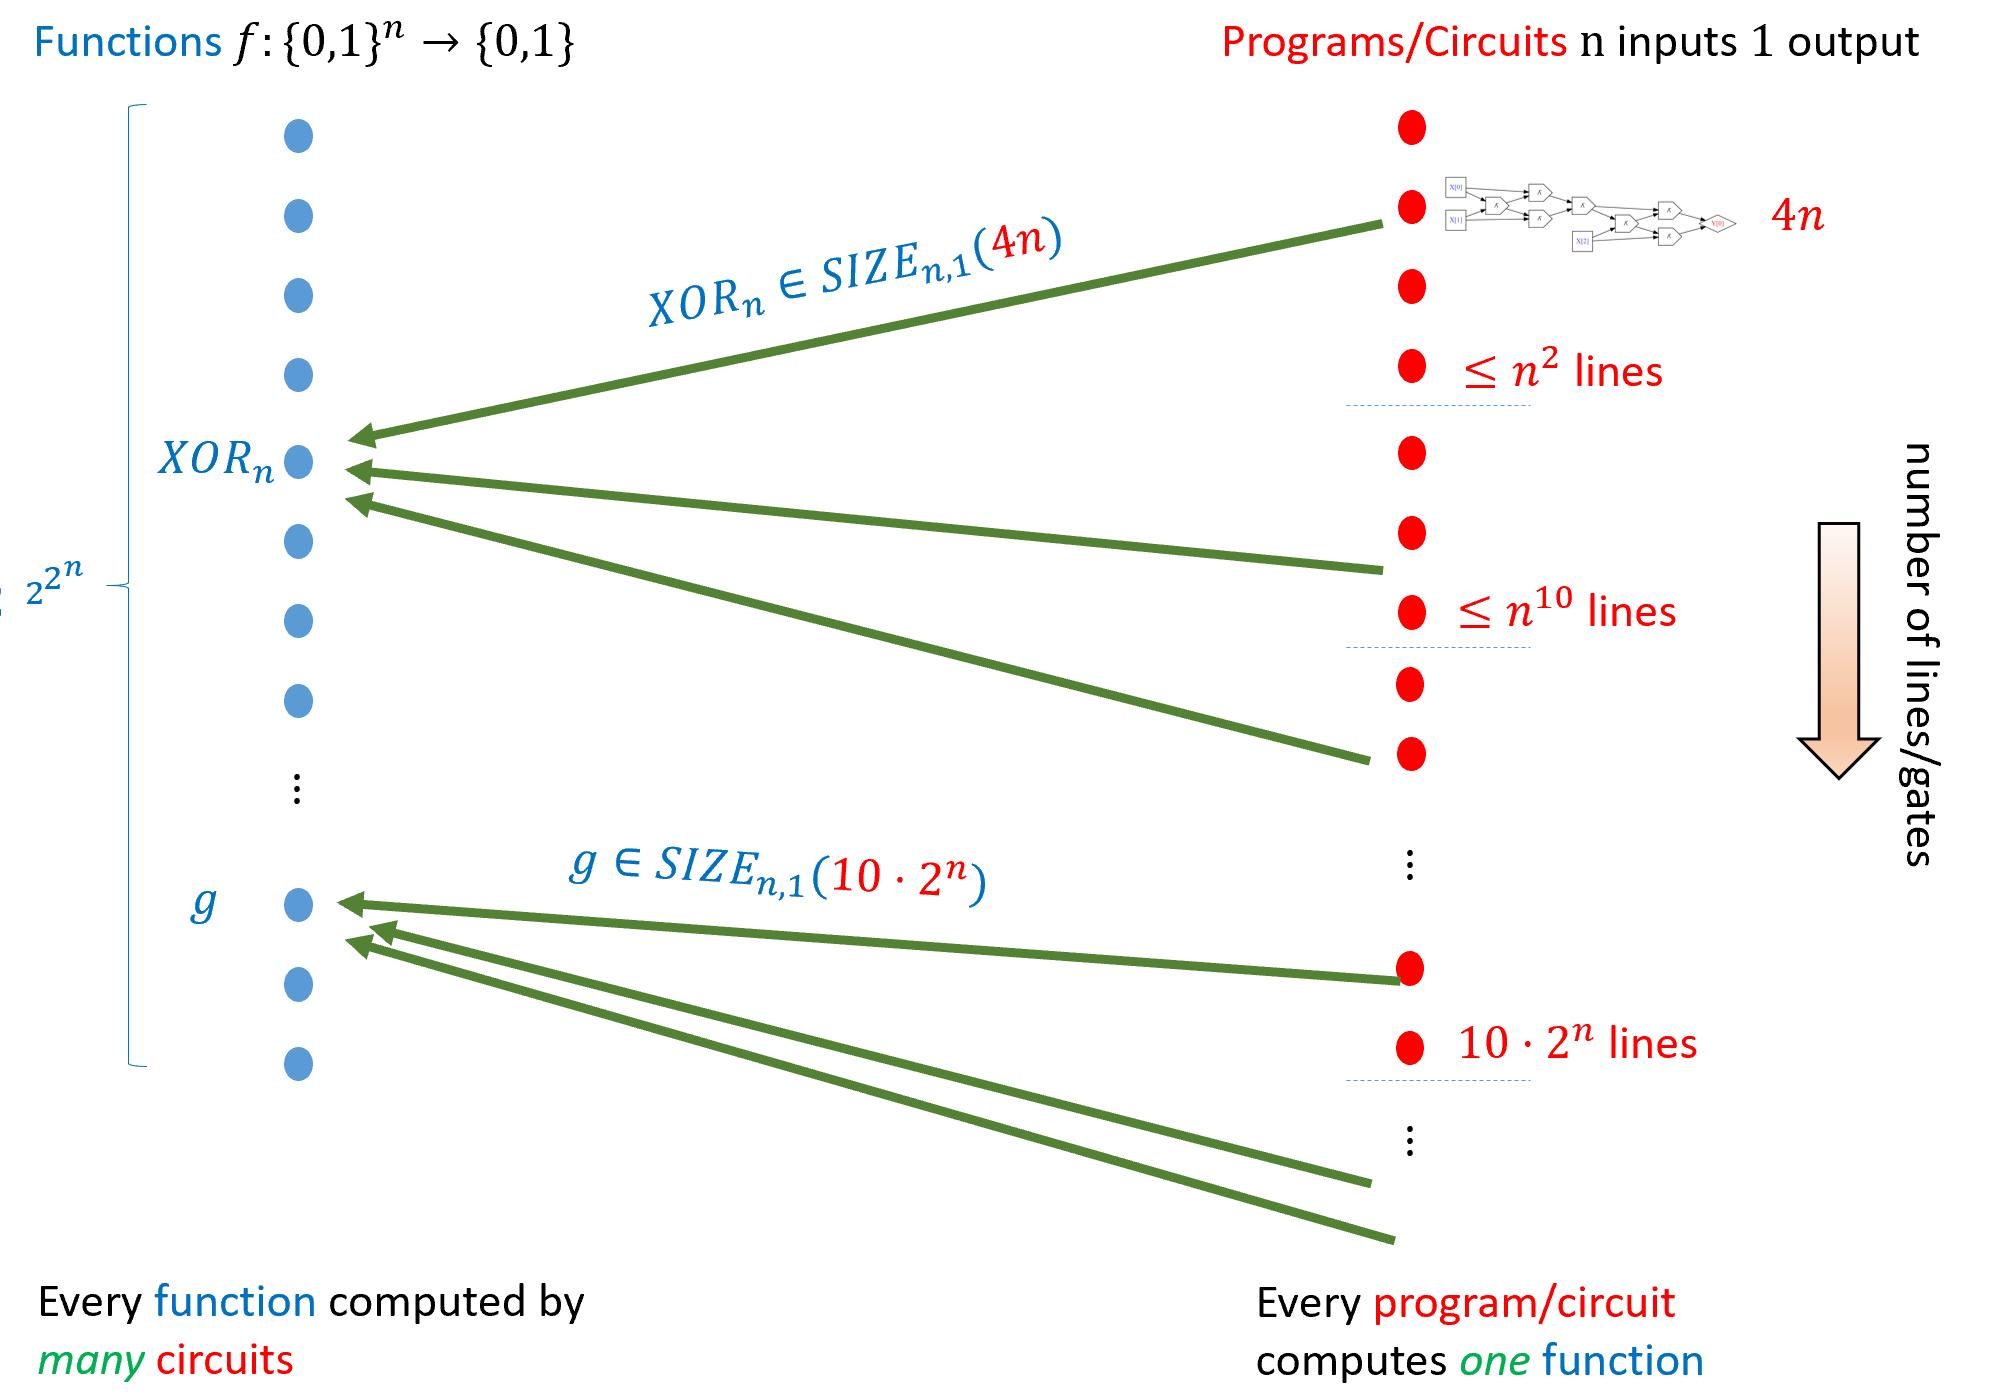
\includegraphics[width=\textwidth, height=0.25\paperheight, keepaspectratio]{../figure/funcvscircs.png}
\caption{There are \(2^{2^n}\) functions mapping \(\{0,1\}^n\) to
\(\{0,1\}\), and an infinite number of circuits with \(n\) bit inputs
and a single bit of output. Every circuit computes one function, but
every function can be computed by many circuits. We say that
\(f \in \ensuremath{\mathit{SIZE}}_{n,1}(s)\) if the smallest circuit
that computes \(f\) has \(s\) or fewer gates. For example
\(\ensuremath{\mathit{XOR}}_n \in \ensuremath{\mathit{SIZE}}_{n,1}(4n)\).
\cref{NAND-univ-thm} shows that \emph{every} function \(g\) is
computable by some circuit of at most \(c\cdot 2^n/n\) gates, and hence
\(\ensuremath{\mathit{SIZE}}_{n,1}(c\cdot 2^n/n)\) corresponds to the
set of \emph{all} functions from \(\{0,1\}^n\) to \(\{0,1\}\).}
\label{funcvscircfig}
\end{figure}

While we defined \(\ensuremath{\mathit{SIZE}}(s)\) with respect to NAND
gates, we would get essentially the same class if we defined it with
respect to AND/OR/NOT gates:

\hypertarget{nandaonsizelem}{}
\begin{lemma} \label[lemma]{nandaonsizelem}

Let \(\ensuremath{\mathit{SIZE}}^{AON}_{n,m}(s)\) denote the set of all
functions \(f:\{0,1\}^n \rightarrow \{0,1\}^m\) that can be computed by
an AND/OR/NOT Boolean circuit of at most \(s\) gates. Then, \[
\ensuremath{\mathit{SIZE}}_{n,m}(s/2) \subseteq \ensuremath{\mathit{SIZE}}^{AON}_{n,m}(s) \subseteq \ensuremath{\mathit{SIZE}}_{n,m}(3s)
\]

\end{lemma}

\begin{proof} \label[proof]{If-f-can-be-computed-by-a}

If \(f\) can be computed by a NAND circuit of at most \(s/2\) gates,
then by replacing each NAND with the two gates NOT and AND, we can
obtain an AND/OR/NOT Boolean circuit of at most \(s\) gates that
computes \(f\). On the other hand, if \(f\) can be computed by a Boolean
AND/OR/NOT circuit of at most \(s\) gates, then by
\cref{NANDuniversamthm} it can be computed by a NAND circuit of at most
\(3s\) gates.

\end{proof}


\begin{marginfigure}
\centering
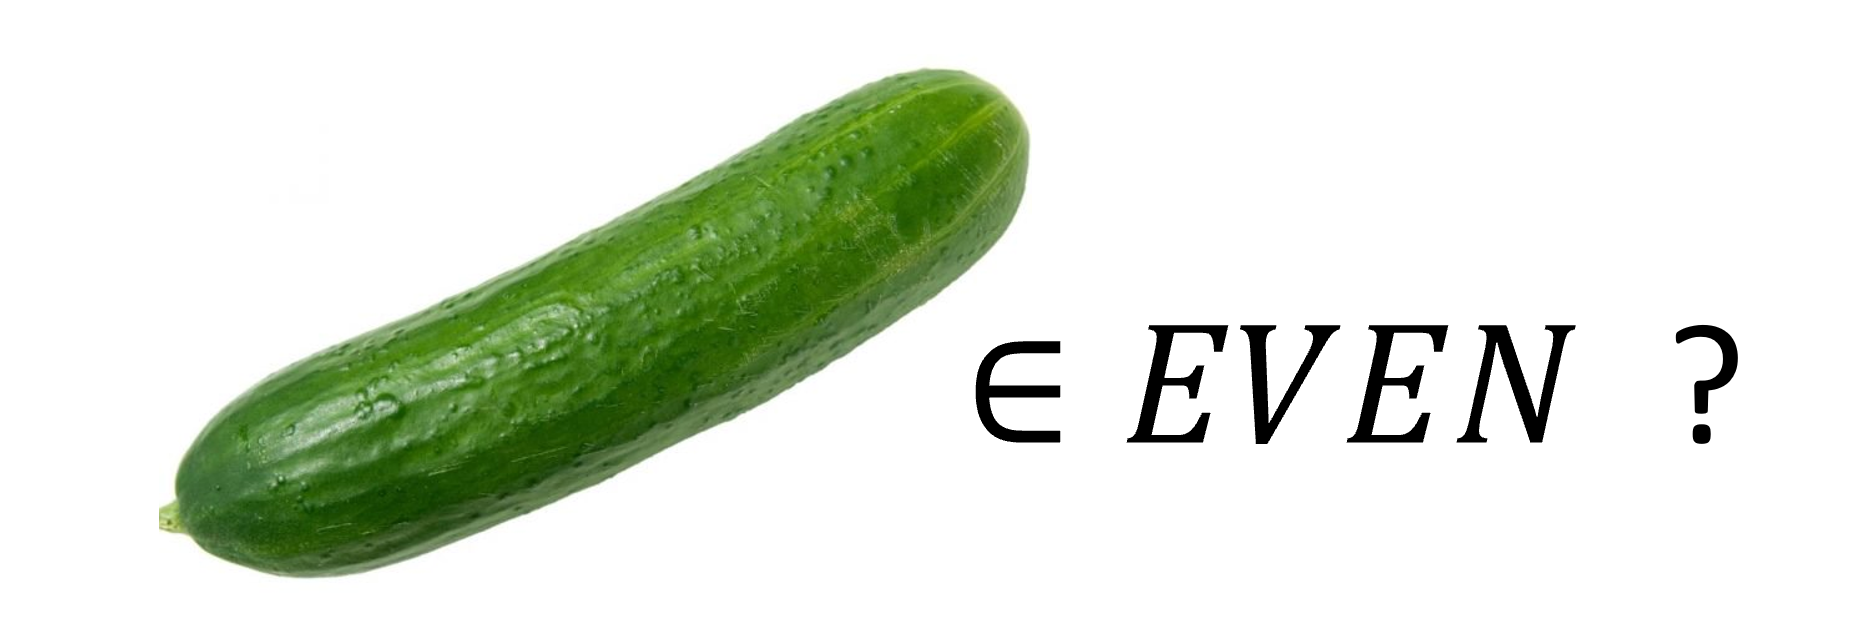
\includegraphics[width=\linewidth, height=1.5in, keepaspectratio]{../figure/cucumber.png}
\caption{A ``category error'' is a question such as ``is a cucumber even
or odd?'' which does not even make sense. In this book one type of
category error you should watch out for is confusing \emph{functions}
and \emph{programs} (i.e., confusing \emph{specifications} and
\emph{implementations}). If \(C\) is a circuit or program, then asking
if \(C \in \ensuremath{\mathit{SIZE}}_{n,1}(s)\) is a category error,
since \(\ensuremath{\mathit{SIZE}}_{n,1}(s)\) is a set of
\emph{functions} and not programs or circuits.}
\label{cucumberfig}
\end{marginfigure}

The results we have seen in this chapter can be phrased as showing that
\(\ensuremath{\mathit{ADD}}_n \in \ensuremath{\mathit{SIZE}}_{2n,n+1}(100 n)\)
and
\(\ensuremath{\mathit{MULT}}_n \in \ensuremath{\mathit{SIZE}}_{2n,2n}(10000 n^{\log_2 3})\).
\cref{NAND-univ-thm} shows that for some constant \(c\),
\(\ensuremath{\mathit{SIZE}}_{n,m}(c m 2^n)\) is equal to the set of all
functions from \(\{0,1\}^n\) to \(\{0,1\}^m\).

\hypertarget{infinitefunc}{}
\begin{remark}[Finite vs infinite functions] \label[remark]{infinitefunc}

A NAND-CIRC program \(P\) can only compute a function with a certain
number \(n\) of inputs and a certain number \(m\) of outputs. Hence, for
example, there is no single NAND-CIRC program that can compute the
increment function
\(\ensuremath{\mathit{INC}}:\{0,1\}^* \rightarrow \{0,1\}^*\) that maps
a string \(x\) (which we identify with a number via the binary
representation) to the string that represents \(x+1\). Rather for every
\(n>0\), there is a NAND-CIRC program \(P_n\) that computes the
restriction \(\ensuremath{\mathit{INC}}_n\) of the function
\(\ensuremath{\mathit{INC}}\) to inputs of length \(n\). Since it can be
shown that for every \(n>0\) such a program \(P_n\) exists of length at
most \(10n\),
\(\ensuremath{\mathit{INC}}_n \in \ensuremath{\mathit{SIZE}}(10n)\) for
every \(n>0\).

If \(T:\N \rightarrow \N\) and \(F:\{0,1\}^* \rightarrow \{0,1\}^*\), we
will write \(F \in \ensuremath{\mathit{SIZE}}_{*}(T(n))\) (or sometimes
slightly abuse notation and write simply
\(F \in \ensuremath{\mathit{SIZE}}(T(n))\)) to indicate that for every
\(n\) the restriction \(F_{\upharpoonright n}\) of \(F\) to inputs in
\(\{0,1\}^n\) is in \(\ensuremath{\mathit{SIZE}}(T(n))\). Hence we can
write
\(\ensuremath{\mathit{INC}} \in \ensuremath{\mathit{SIZE}}_*(10n)\). We
will come back to this issue of finite vs infinite functions later in
this course.

\end{remark}

\hypertarget{sizeclosundercomp}{}
\begin{solvedexercise}[$SIZE$ closed under complement.] \label[solvedexercise]{sizeclosundercomp}

In this exercise we prove a certain ``closure property'' of the class
\(\ensuremath{\mathit{SIZE}}_n(s)\). That is, we show that if \(f\) is
in this class then (up to some small additive term) so is the complement
of \(f\), which is the function \(g(x)=1-f(x)\).

Prove that there is a constant \(c\) such that for every
\(f:\{0,1\}^n \rightarrow \{0,1\}\) and \(s\in \N\), if
\(f \in \ensuremath{\mathit{SIZE}}_n(s)\) then
\(1-f \in \ensuremath{\mathit{SIZE}}_n(s+c)\).

\end{solvedexercise}

\begin{solution} \label[solution]{If-fin-ensuremathmathitSI}

If \(f\in \ensuremath{\mathit{SIZE}}(s)\) then there is an \(s\)-line
NAND-CIRC program \(P\) that computes \(f\). We can rename the variable
\texttt{Y[0]} in \(P\) to a variable \texttt{temp} and add the line

\begin{code}
Y[0] = NAND(temp,temp)
\end{code}

at the very end to obtain a program \(P'\) that computes \(1-f\).

\end{solution}

\begin{recap} \label[recap]{We-can-define-the-notion-}

\begin{itemize}
\tightlist
\item
  We can define the notion of computing a function via a simplified
  ``programming language'', where computing a function \(F\) in \(T\)
  steps would correspond to having a \(T\)-line NAND-CIRC program that
  computes \(F\).
\item
  While the NAND-CIRC programming only has one operation, other
  operations such as functions and conditional execution can be
  implemented using it.
\item
  Every function \(f:\{0,1\}^n \rightarrow \{0,1\}^m\) can be computed
  by a circuit of at most \(O(m 2^n)\) gates (and in fact at most
  \(O(m 2^n/n)\) gates).
\item
  Sometimes (or maybe always?) we can translate an \emph{efficient}
  algorithm to compute \(f\) into a circuit that computes \(f\) with a
  number of gates comparable to the number of steps in this algorithm.
\end{itemize}

\end{recap}

\section{Exercises}\label{Exercises}

\hypertarget{embedtuples-ex}{}
\begin{exercise}[Pairing] \label[exercise]{embedtuples-ex}

This exercise asks you to give a one-to-one map from \(\N^2\) to \(\N\).
This can be useful to implement two-dimensional arrays as ``syntactic
sugar'' in programming languages that only have one-dimensional array.

\begin{enumerate}
\def\labelenumi{\arabic{enumi}.}
\item
  Prove that the map \(F(x,y)=2^x3^y\) is a one-to-one map from \(\N^2\)
  to \(\N\).
\item
  Show that there is a one-to-one map \(F:\N^2 \rightarrow \N\) such
  that for every \(x,y\), \(F(x,y) \leq 100\cdot \max\{x,y\}^2+100\).
\item
  For every \(k\), show that there is a one-to-one map
  \(F:\N^k \rightarrow \N\) such that for every
  \(x_0,\ldots,x_{k-1} \in \N\),
  \(F(x_0,\ldots,x_{k-1}) \leq 100 \cdot (x_0+x_1+\ldots+x_{k-1}+100k)^k\).
\end{enumerate}

\end{exercise}

\hypertarget{mux-ex}{}
\begin{exercise}[Computing MUX] \label[exercise]{mux-ex}

Prove that the NAND-CIRC program below computes the function
\(\ensuremath{\mathit{MUX}}\) (or \(\ensuremath{\mathit{LOOKUP}}_1\))
where \(\ensuremath{\mathit{MUX}}(a,b,c)\) equals \(a\) if \(c=0\) and
equals \(b\) if \(c=1\):

\begin{code}
t = NAND(X[2],X[2])
u = NAND(X[0],t)
v = NAND(X[1],X[2])
Y[0] = NAND(u,v)
\end{code}

\end{exercise}

\hypertarget{atleasttwo-ex}{}
\begin{exercise}[At least two / Majority] \label[exercise]{atleasttwo-ex}

Give a NAND-CIRC program of at most 6 lines to compute the function
\(\ensuremath{\mathit{MAJ}}:\{0,1\}^3 \rightarrow \{0,1\}\) where
\(\ensuremath{\mathit{MAJ}}(a,b,c) = 1\) iff \(a+b+c \geq 2\).

\end{exercise}

\hypertarget{conditionalsugarthmex}{}
\begin{exercise}[Conditional statements] \label[exercise]{conditionalsugarthmex}

In this exercise we will explore \cref{conditionalsugarthm}:
transforming NAND-CIRC-IF programs that use code such as
\texttt{if .. then .. else ..} to standard NAND-CIRC programs.

\begin{enumerate}
\def\labelenumi{\arabic{enumi}.}
\item
  Give a ``proof by code'' of \cref{conditionalsugarthm}: a program in a
  programming language of your choice that transforms a NAND-CIRC-IF
  program \(P\) into a ``sugar free'' NAND-CIRC program \(P'\) that
  computes the same function. See footnote for hint.\footnote{You can
    start by transforming \(P\) into a NAND-CIRC-PROC program that uses
    procedure statements, and then use the code of \cref{desugarcode} to
    transform the latter into a ``sugar free'' NAND-CIRC program.}
\item
  Prove the following statement, which is the heart of
  \cref{conditionalsugarthm}: suppose that there exists an \(s\)-line
  NAND-CIRC program to compute \(f:\{0,1\}^n \rightarrow \{0,1\}\) and
  an \(s'\)-line NAND-CIRC program to compute
  \(g:\{0,1\}^n \rightarrow \{0,1\}\). Prove that there exist a
  NAND-CIRC program of at most \(s+s'+10\) lines to compute the function
  \(h:\{0,1\}^{n+1} \rightarrow \{0,1\}\) where
  \(h(x_0,\ldots,x_{n-1},x_n)\) equals \(f(x_0,\ldots,x_{n-1})\) if
  \(x_n=0\) and equals \(g(x_0,\ldots,x_{n-1})\) otherwise. (All
  programs in this item are standard ``sugar-free'' NAND-CIRC programs.)
\end{enumerate}

\end{exercise}

\hypertarget{halffulladderex}{}
\begin{exercise}[Half and full adders] \label[exercise]{halffulladderex}

\begin{enumerate}
\def\labelenumi{\arabic{enumi}.}
\item
  A \emph{half adder} is the function
  \(\ensuremath{\mathit{HA}}:\{0,1\}^2 :\rightarrow \{0,1\}^2\) that
  corresponds to adding two binary bits. That is, for every
  \(a,b \in \{0,1\}\), \(\ensuremath{\mathit{HA}}(a,b)= (e,f)\) where
  \(2e+f = a+b\). Prove that there is a NAND circuit of at most five
  NAND gates that computes \(\ensuremath{\mathit{HA}}\).
\item
  A \emph{full adder} is the function
  \(\ensuremath{\mathit{FA}}:\{0,1\}^3 \rightarrow \{0,1\}^{2}\) that
  takes in two bits and a ``carry'' bit and outputs their sum. That is,
  for every \(a,b,c \in \{0,1\}\),
  \(\ensuremath{\mathit{FA}}(a,b,c) = (e,f)\) such that
  \(2e+f = a+b+c\). Prove that there is a NAND circuit of at most nine
  NAND gates that computes \(\ensuremath{\mathit{FA}}\).
\item
  Prove that if there is a NAND circuit of \(c\) gates that computes
  \(\ensuremath{\mathit{FA}}\), then there is a circuit of \(cn\) gates
  that computes \(\ensuremath{\mathit{ADD}}_n\) where (as in
  \cref{addition-thm})
  \(\ensuremath{\mathit{ADD}}_n:\{0,1\}^{2n} \rightarrow \{0,1\}^{n+1}\)
  is the function that outputs the addition of two input \(n\)-bit
  numbers. See footnote for hint.\footnote{Use a ``cascade'' of adding
    the bits one after the other, starting with the least significant
    digit, just like in the elementary-school algorithm.}
\item
  Show that for every \(n\) there is a NAND-CIRC program to compute
  \(\ensuremath{\mathit{ADD}}_n\) with at most \(9n\) lines.
\end{enumerate}

\end{exercise}

\hypertarget{addition-ex}{}
\begin{exercise}[Addition] \label[exercise]{addition-ex}

Write a program using your favorite programming language that on input
of an integer \(n\), outputs a NAND-CIRC program that computes
\(\ensuremath{\mathit{ADD}}_n\). Can you ensure that the program it
outputs for \(\ensuremath{\mathit{ADD}}_n\) has fewer than \(10n\)
lines?

\end{exercise}

\hypertarget{multiplication-ex}{}
\begin{exercise}[Multiplication] \label[exercise]{multiplication-ex}

Write a program using your favorite programming language that on input
of an integer \(n\), outputs a NAND-CIRC program that computes
\(\ensuremath{\mathit{MULT}}_n\). Can you ensure that the program it
outputs for \(\ensuremath{\mathit{MULT}}_n\) has fewer than
\(1000\cdot n^2\) lines?

\end{exercise}

\hypertarget{eff-multiplication-ex}{}
\begin{exercise}[Efficient multiplication (challenge)] \label[exercise]{eff-multiplication-ex}

Write a program using your favorite programming language that on input
of an integer \(n\), outputs a NAND-CIRC program that computes
\(\ensuremath{\mathit{MULT}}_n\) and has at most \(10000 n^{1.9}\)
lines.\footnote{\textbf{Hint:} Use Karatsuba's algorithm.} What is the
smallest number of lines you can use to multiply two 2048 bit numbers?

\end{exercise}

\hypertarget{mult-bit-ex}{}
\begin{exercise}[Multibit function] \label[exercise]{mult-bit-ex}

In the text \cref{NAND-univ-thm} is only proven for the case \(m=1\). In
this exercise you will extend the proof for every \(m\).

Prove that

\begin{enumerate}
\def\labelenumi{\arabic{enumi}.}
\item
  If there is an \(s\)-line NAND-CIRC program to compute
  \(f:\{0,1\}^n \rightarrow \{0,1\}\) and an \(s'\)-line NAND-CIRC
  program to compute \(f':\{0,1\}^n \rightarrow \{0,1\}\) then there is
  an \(s+s'\)-line program to compute the function
  \(g:\{0,1\}^n \rightarrow \{0,1\}^2\) such that \(g(x)=(f(x),f'(x))\).
\item
  For every function \(f:\{0,1\}^n \rightarrow \{0,1\}^m\), there is a
  NAND-CIRC program of at most \(10m\cdot 2^n\) lines that computes
  \(f\). (You can use the \(m=1\) case of \cref{NAND-univ-thm}, as well
  as Item 1.)
\end{enumerate}

\end{exercise}

\hypertarget{usesugarex}{}
\begin{exercise}[Simplifying using syntactic sugar] \label[exercise]{usesugarex}

Let \(P\) be the following NAND-CIRC program:

\begin{code}
Temp[0] = NAND(X[0],X[0])
Temp[1] = NAND(X[1],X[1])
Temp[2] = NAND(Temp[0],Temp[1])
Temp[3] = NAND(X[2],X[2])
Temp[4] = NAND(X[3],X[3])
Temp[5] = NAND(Temp[3],Temp[4])
Temp[6] = NAND(Temp[2],Temp[2])
Temp[7] = NAND(Temp[5],Temp[5])
Y[0] = NAND(Temp[6],Temp[7])
\end{code}

\begin{enumerate}
\def\labelenumi{\arabic{enumi}.}
\item
  Write a program \(P'\) with at most three lines of code that uses both
  \texttt{NAND} as well as the syntactic sugar \texttt{OR} that computes
  the same function as \(P\).
\item
  Draw a circuit that computes the same function as \(P\) and uses only
  \(\ensuremath{\mathit{AND}}\) and \(\ensuremath{\mathit{NOT}}\) gates.
\end{enumerate}

\end{exercise}

In the following exercises you are asked to compare the \emph{power} of
pairs programming languages. By ``comparing the power'' of two
programming languages \(X\) and \(Y\) we mean determining the relation
between the set of functions that are computable using programs in \(X\)
and \(Y\) respectively. That is, to answer such a question you need to
do both of the following:

\begin{enumerate}
\def\labelenumi{\arabic{enumi}.}
\tightlist
\item
  Either prove that for every program \(P\) in \(X\) there is a program
  \(P'\) in \(Y\) that computes the same function as \(P\), \emph{or}
  give an example for a function that is computable by an \(X\)-program
  but not computable by a \(Y\)-program.
\end{enumerate}

\emph{and}

\begin{enumerate}
\def\labelenumi{\arabic{enumi}.}
\tightlist
\item
  Either prove that for every program \(P\) in \(Y\) there is a program
  \(P'\) in \(X\) that computes the same function as \(P\), \emph{or}
  give an example for a function that is computable by a \(Y\)-program
  but not computable by an \(X\)-program.
\end{enumerate}

When you give an example as above of a function that is computable in
one programming language but not the other, you need to \emph{prove}
that the function you showed is \emph{(1)} computable in the first
programming language and \emph{(2)} \emph{not computable} in the second
programming language.

\hypertarget{compareif}{}
\begin{exercise}[Compare IF and NAND] \label[exercise]{compareif}

Let IF-CIRC be the programming language where we have the following
operations \texttt{foo = 0}, \texttt{foo = 1},
\texttt{foo = IF(cond,yes,no)} (that is, we can use the constants \(0\)
and \(1\), and the
\(\ensuremath{\mathit{IF}}:\{0,1\}^3 \rightarrow \{0,1\}\) function such
that \(\ensuremath{\mathit{IF}}(a,b,c)\) equals \(b\) if \(a=1\) and
equals \(c\) if \(a=0\)). Compare the power of the NAND-CIRC programming
language and the IF-CIRC programming language.

\end{exercise}

\hypertarget{comparexor}{}
\begin{exercise}[Compare XOR and NAND] \label[exercise]{comparexor}

Let XOR-CIRC be the programming language where we have the following
operations \texttt{foo = XOR(bar,blah)}, \texttt{foo = 1} and
\texttt{bar = 0} (that is, we can use the constants \(0\), \(1\) and the
\(\ensuremath{\mathit{XOR}}\) function that maps \(a,b \in \{0,1\}^2\)
to \(a+b \mod 2\)). Compare the power of the NAND-CIRC programming
language and the XOR-CIRC programming language. See footnote for
hint.\footnote{You can use the fact that
  \((a+b)+c \mod 2 = a+b+c \mod 2\). In particular it means that if you
  have the lines \texttt{d = XOR(a,b)} and \texttt{e = XOR(d,c)} then
  \texttt{e} gets the sum modulo \(2\) of the variable \texttt{a},
  \texttt{b} and \texttt{c}.}

\end{exercise}

\hypertarget{majasymp}{}
\begin{exercise}[Circuits for majority] \label[exercise]{majasymp}

Prove that there is some constant \(c\) such that for every \(n>1\),
\(\ensuremath{\mathit{MAJ}}_n \in Size(cn)\) where
\(\ensuremath{\mathit{MAJ}}_n:\{0,1\}^n \rightarrow \{0,1\}\) is the
majority function on \(n\) input bits. That is
\(\ensuremath{\mathit{MAJ}}_n(x)=1\) iff \(\sum_{i=0}^{n-1}x_i > n/2\).
See footnote for hint.\footnote{One approach to solve this is using
  recursion and the so-called
  \href{https://en.wikipedia.org/wiki/Master\%5Ftheorem\%5F(analysis\%5Fof\%5Falgorithms)}{Master
  Theorem}.}

\end{exercise}

\hypertarget{thresholdcirc}{}
\begin{exercise}[Circuits for threshold] \label[exercise]{thresholdcirc}

Prove that there is some constant \(c\) such that for every \(n>1\), and
integers
\(a_0,\ldots,a_{n-1},b \in \{-2^n,-2^n+1,\ldots,-1,0,+1,\ldots,2^n\}\),
there is a NAND circuit with at most \(n^c\) gates that computes the
\emph{threshold} function
\(f_{a_0,\ldots,a_{n-1},b}:\{0,1\}^n \rightarrow \{0,1\}\) that on input
\(x\in \{0,1\}^n\) outputs \(1\) if and only if
\(\sum_{i=0}^{n-1} a_i x_i > b\).

\end{exercise}

\section{Bibliographical notes}\label{computeeveryfunctionbibnotes}

See Jukna's and Wegener's books \cite{Jukna12, wegener1987complexity}
for much more extensive discussion on circuits. Shannon showed that
every Boolean function can be computed by a circuit of exponential size
\cite{Shannon1938}. The improved bound of \(c \cdot 2^n/n\) (with the
optimal value of \(c\) for many bases) is due to Lupanov
\cite{Lupanov1958}. An exposition of this for the case of NAND (where
\(c=1\)) is given in Chapter 4 of his book \cite{lupanov1984}. (Thanks
to Sasha Golovnev for tracking down this reference!)

The concept of ``syntactic sugar'' is also known as ``macros'' or
``meta-programming'' and is sometimes implemented via a preprocessor or
macro language in a programming language or a text editor. One modern
example is the \href{https://babeljs.io/}{Babel} JavaScript syntax
transformer, that converts JavaScript programs written using the latest
features into a format that older Browsers can accept. It even has a
\href{https://babeljs.io/docs/plugins/}{plug-in} architecture, that
allows users to add their own syntactic sugar to the language.
